% Options for packages loaded elsewhere
\PassOptionsToPackage{unicode}{hyperref}
\PassOptionsToPackage{hyphens}{url}
%
\documentclass[
]{article}
\usepackage{lmodern}
\usepackage{amsmath}
\usepackage{ifxetex,ifluatex}
\ifnum 0\ifxetex 1\fi\ifluatex 1\fi=0 % if pdftex
  \usepackage[T1]{fontenc}
  \usepackage[utf8]{inputenc}
  \usepackage{textcomp} % provide euro and other symbols
  \usepackage{amssymb}
\else % if luatex or xetex
  \usepackage{unicode-math}
  \defaultfontfeatures{Scale=MatchLowercase}
  \defaultfontfeatures[\rmfamily]{Ligatures=TeX,Scale=1}
\fi
% Use upquote if available, for straight quotes in verbatim environments
\IfFileExists{upquote.sty}{\usepackage{upquote}}{}
\IfFileExists{microtype.sty}{% use microtype if available
  \usepackage[]{microtype}
  \UseMicrotypeSet[protrusion]{basicmath} % disable protrusion for tt fonts
}{}
\makeatletter
\@ifundefined{KOMAClassName}{% if non-KOMA class
  \IfFileExists{parskip.sty}{%
    \usepackage{parskip}
  }{% else
    \setlength{\parindent}{0pt}
    \setlength{\parskip}{6pt plus 2pt minus 1pt}}
}{% if KOMA class
  \KOMAoptions{parskip=half}}
\makeatother
\usepackage{xcolor}
\IfFileExists{xurl.sty}{\usepackage{xurl}}{} % add URL line breaks if available
\IfFileExists{bookmark.sty}{\usepackage{bookmark}}{\usepackage{hyperref}}
\hypersetup{
  pdftitle={590 HW1},
  pdfauthor={Austin Turvy Derek Holste Mason Carhart},
  hidelinks,
  pdfcreator={LaTeX via pandoc}}
\urlstyle{same} % disable monospaced font for URLs
\usepackage[margin=1in]{geometry}
\usepackage{color}
\usepackage{fancyvrb}
\newcommand{\VerbBar}{|}
\newcommand{\VERB}{\Verb[commandchars=\\\{\}]}
\DefineVerbatimEnvironment{Highlighting}{Verbatim}{commandchars=\\\{\}}
% Add ',fontsize=\small' for more characters per line
\usepackage{framed}
\definecolor{shadecolor}{RGB}{248,248,248}
\newenvironment{Shaded}{\begin{snugshade}}{\end{snugshade}}
\newcommand{\AlertTok}[1]{\textcolor[rgb]{0.94,0.16,0.16}{#1}}
\newcommand{\AnnotationTok}[1]{\textcolor[rgb]{0.56,0.35,0.01}{\textbf{\textit{#1}}}}
\newcommand{\AttributeTok}[1]{\textcolor[rgb]{0.77,0.63,0.00}{#1}}
\newcommand{\BaseNTok}[1]{\textcolor[rgb]{0.00,0.00,0.81}{#1}}
\newcommand{\BuiltInTok}[1]{#1}
\newcommand{\CharTok}[1]{\textcolor[rgb]{0.31,0.60,0.02}{#1}}
\newcommand{\CommentTok}[1]{\textcolor[rgb]{0.56,0.35,0.01}{\textit{#1}}}
\newcommand{\CommentVarTok}[1]{\textcolor[rgb]{0.56,0.35,0.01}{\textbf{\textit{#1}}}}
\newcommand{\ConstantTok}[1]{\textcolor[rgb]{0.00,0.00,0.00}{#1}}
\newcommand{\ControlFlowTok}[1]{\textcolor[rgb]{0.13,0.29,0.53}{\textbf{#1}}}
\newcommand{\DataTypeTok}[1]{\textcolor[rgb]{0.13,0.29,0.53}{#1}}
\newcommand{\DecValTok}[1]{\textcolor[rgb]{0.00,0.00,0.81}{#1}}
\newcommand{\DocumentationTok}[1]{\textcolor[rgb]{0.56,0.35,0.01}{\textbf{\textit{#1}}}}
\newcommand{\ErrorTok}[1]{\textcolor[rgb]{0.64,0.00,0.00}{\textbf{#1}}}
\newcommand{\ExtensionTok}[1]{#1}
\newcommand{\FloatTok}[1]{\textcolor[rgb]{0.00,0.00,0.81}{#1}}
\newcommand{\FunctionTok}[1]{\textcolor[rgb]{0.00,0.00,0.00}{#1}}
\newcommand{\ImportTok}[1]{#1}
\newcommand{\InformationTok}[1]{\textcolor[rgb]{0.56,0.35,0.01}{\textbf{\textit{#1}}}}
\newcommand{\KeywordTok}[1]{\textcolor[rgb]{0.13,0.29,0.53}{\textbf{#1}}}
\newcommand{\NormalTok}[1]{#1}
\newcommand{\OperatorTok}[1]{\textcolor[rgb]{0.81,0.36,0.00}{\textbf{#1}}}
\newcommand{\OtherTok}[1]{\textcolor[rgb]{0.56,0.35,0.01}{#1}}
\newcommand{\PreprocessorTok}[1]{\textcolor[rgb]{0.56,0.35,0.01}{\textit{#1}}}
\newcommand{\RegionMarkerTok}[1]{#1}
\newcommand{\SpecialCharTok}[1]{\textcolor[rgb]{0.00,0.00,0.00}{#1}}
\newcommand{\SpecialStringTok}[1]{\textcolor[rgb]{0.31,0.60,0.02}{#1}}
\newcommand{\StringTok}[1]{\textcolor[rgb]{0.31,0.60,0.02}{#1}}
\newcommand{\VariableTok}[1]{\textcolor[rgb]{0.00,0.00,0.00}{#1}}
\newcommand{\VerbatimStringTok}[1]{\textcolor[rgb]{0.31,0.60,0.02}{#1}}
\newcommand{\WarningTok}[1]{\textcolor[rgb]{0.56,0.35,0.01}{\textbf{\textit{#1}}}}
\usepackage{graphicx}
\makeatletter
\def\maxwidth{\ifdim\Gin@nat@width>\linewidth\linewidth\else\Gin@nat@width\fi}
\def\maxheight{\ifdim\Gin@nat@height>\textheight\textheight\else\Gin@nat@height\fi}
\makeatother
% Scale images if necessary, so that they will not overflow the page
% margins by default, and it is still possible to overwrite the defaults
% using explicit options in \includegraphics[width, height, ...]{}
\setkeys{Gin}{width=\maxwidth,height=\maxheight,keepaspectratio}
% Set default figure placement to htbp
\makeatletter
\def\fps@figure{htbp}
\makeatother
\setlength{\emergencystretch}{3em} % prevent overfull lines
\providecommand{\tightlist}{%
  \setlength{\itemsep}{0pt}\setlength{\parskip}{0pt}}
\setcounter{secnumdepth}{-\maxdimen} % remove section numbering
\usepackage{booktabs}
\usepackage{longtable}
\usepackage{array}
\usepackage{multirow}
\usepackage{wrapfig}
\usepackage{float}
\usepackage{colortbl}
\usepackage{pdflscape}
\usepackage{tabu}
\usepackage{threeparttable}
\usepackage{threeparttablex}
\usepackage[normalem]{ulem}
\usepackage{makecell}
\usepackage{xcolor}
\ifluatex
  \usepackage{selnolig}  % disable illegal ligatures
\fi

\title{590 HW1}
\author{Austin Turvy Derek Holste Mason Carhart}
\date{4/13/2021}

\begin{document}
\maketitle

\begin{Shaded}
\begin{Highlighting}[]
\CommentTok{\# Load packages}
\FunctionTok{library}\NormalTok{(pacman)}
\FunctionTok{p\_load}\NormalTok{(readr, data.table, dplyr, janitor, haven, here, }
\NormalTok{       tidyverse, skimr, lfe, stargazer, quantreg, hrbrthemes, }
\NormalTok{       tinytex, kableExtra, broom)}
\end{Highlighting}
\end{Shaded}

\begin{Shaded}
\begin{Highlighting}[]
\CommentTok{\# Load data}
\NormalTok{af }\OtherTok{=} \FunctionTok{read\_dta}\NormalTok{(}\FunctionTok{here}\NormalTok{(}\StringTok{"afghanistan\_anonymized\_data.dta"}\NormalTok{)) }
\end{Highlighting}
\end{Shaded}

\begin{Shaded}
\begin{Highlighting}[]
\CommentTok{\# Create nonoutlier column}
\NormalTok{af }\OtherTok{\textless{}{-}}\NormalTok{ af }\SpecialCharTok{\%\textgreater{}\%} \FunctionTok{mutate}\NormalTok{(}\AttributeTok{nonoutlier=} \FunctionTok{ifelse}\NormalTok{((f07\_num\_ppl\_hh\_cnt }\SpecialCharTok{\textgreater{}} \DecValTok{20} \SpecialCharTok{\&}\NormalTok{ f07\_observed }\SpecialCharTok{==} \DecValTok{1}\NormalTok{) }\SpecialCharTok{|}
\NormalTok{                                    (f07\_jeribs\_cnt }\SpecialCharTok{\textgreater{}} \DecValTok{10} \SpecialCharTok{\&}\NormalTok{ f07\_observed }\SpecialCharTok{==} \DecValTok{1}\NormalTok{)}\SpecialCharTok{|}
\NormalTok{                                    (f07\_num\_sheep\_cnt }\SpecialCharTok{\textgreater{}} \DecValTok{50} \SpecialCharTok{\&}\NormalTok{ f07\_observed }\SpecialCharTok{==} \DecValTok{1}\NormalTok{)}\SpecialCharTok{|}
\NormalTok{                                      (s08\_num\_ppl\_hh\_cnt }\SpecialCharTok{\textgreater{}} \DecValTok{20} \SpecialCharTok{\&}\NormalTok{ s08\_observed }\SpecialCharTok{==} \DecValTok{1}\NormalTok{)}\SpecialCharTok{|}
\NormalTok{                                      (s08\_jeribs\_cnt }\SpecialCharTok{\textgreater{}} \DecValTok{10} \SpecialCharTok{\&}\NormalTok{ s08\_observed }\SpecialCharTok{==} \DecValTok{1}\NormalTok{) }\SpecialCharTok{|}
\NormalTok{                                      (s08\_num\_sheep\_cnt }\SpecialCharTok{\textgreater{}} \DecValTok{50} \SpecialCharTok{\&}\NormalTok{ s08\_observed }\SpecialCharTok{==} \DecValTok{1}\NormalTok{)}
\NormalTok{                                      ,}\DecValTok{0}\NormalTok{,}\DecValTok{1}\NormalTok{))}


\CommentTok{\# Tabulating nonoutliers}
\NormalTok{non\_outlier\_tab }\OtherTok{\textless{}{-}}\NormalTok{ af }\SpecialCharTok{\%\textgreater{}\%} \FunctionTok{group\_by}\NormalTok{(nonoutlier) }\SpecialCharTok{\%\textgreater{}\%} 
    \FunctionTok{summarise}\NormalTok{(}\AttributeTok{count =} \FunctionTok{n}\NormalTok{(), }\AttributeTok{percentage =} \FunctionTok{n}\NormalTok{()}\SpecialCharTok{/}\FunctionTok{nrow}\NormalTok{(.))}

\NormalTok{non\_outlier\_tab}
\end{Highlighting}
\end{Shaded}

\begin{verbatim}
## # A tibble: 2 x 3
##   nonoutlier count percentage
##        <dbl> <int>      <dbl>
## 1          0    76     0.0421
## 2          1  1728     0.958
\end{verbatim}

There are 76 non-outliers in the data given the specifications prior.

\begin{Shaded}
\begin{Highlighting}[]
\CommentTok{\# Run girls regression table 4 column 1 including outliers}
\NormalTok{reg3 }\OtherTok{=} \FunctionTok{felm}\NormalTok{(f07\_formal\_school }\SpecialCharTok{\textasciitilde{}}\NormalTok{ treatment }\SpecialCharTok{+}\NormalTok{ chagcharan }\SpecialCharTok{|} \DecValTok{0} \SpecialCharTok{|} \DecValTok{0} \SpecialCharTok{|}\NormalTok{ clustercode, }
            \AttributeTok{data =}\NormalTok{ af }\SpecialCharTok{\%\textgreater{}\%} \FunctionTok{filter}\NormalTok{(f07\_girl\_cnt }\SpecialCharTok{==} \DecValTok{1} \SpecialCharTok{\&} 
\NormalTok{                                 f07\_observed }\SpecialCharTok{==} \DecValTok{1}\NormalTok{))}

\CommentTok{\# Run boys regression table 4 column 1including outliers}
\NormalTok{reg4 }\OtherTok{=} \FunctionTok{felm}\NormalTok{(f07\_formal\_school }\SpecialCharTok{\textasciitilde{}}\NormalTok{ treatment }\SpecialCharTok{+}\NormalTok{ chagcharan }\SpecialCharTok{|} \DecValTok{0} \SpecialCharTok{|} \DecValTok{0} \SpecialCharTok{|}\NormalTok{ clustercode, }
            \AttributeTok{data =}\NormalTok{ af }\SpecialCharTok{\%\textgreater{}\%} \FunctionTok{filter}\NormalTok{(f07\_girl\_cnt }\SpecialCharTok{==} \DecValTok{0} \SpecialCharTok{\&} 
\NormalTok{                                 f07\_observed }\SpecialCharTok{==} \DecValTok{1}\NormalTok{))}
\end{Highlighting}
\end{Shaded}

\begin{Shaded}
\begin{Highlighting}[]
\CommentTok{\# Run girls regression table 4 column 1 with controls}
\NormalTok{reg5 }\OtherTok{=} \FunctionTok{felm}\NormalTok{(f07\_formal\_school }\SpecialCharTok{\textasciitilde{}}\NormalTok{ treatment }\SpecialCharTok{+}\NormalTok{ chagcharan }\SpecialCharTok{+}\NormalTok{ f07\_heads\_child\_cnt }\SpecialCharTok{+} 
\NormalTok{              f07\_age\_cnt }\SpecialCharTok{+}\NormalTok{ f07\_duration\_village\_cnt }\SpecialCharTok{+} 
\NormalTok{              f07\_farsi\_cnt }\SpecialCharTok{+}\NormalTok{ f07\_tajik\_cnt }\SpecialCharTok{+}\NormalTok{ f07\_farmer\_cnt }\SpecialCharTok{+} 
\NormalTok{              f07\_age\_head\_cnt }\SpecialCharTok{+}\NormalTok{ f07\_yrs\_ed\_head\_cnt }\SpecialCharTok{+}\NormalTok{ f07\_num\_ppl\_hh\_cnt }\SpecialCharTok{+} 
\NormalTok{              f07\_jeribs\_cnt }\SpecialCharTok{+}\NormalTok{ f07\_num\_sheep\_cnt }\SpecialCharTok{+} 
\NormalTok{              f07\_nearest\_scl}\SpecialCharTok{|} \DecValTok{0} \SpecialCharTok{|} \DecValTok{0} \SpecialCharTok{|}\NormalTok{ clustercode, }
            \AttributeTok{data =}\NormalTok{ af }\SpecialCharTok{\%\textgreater{}\%} \FunctionTok{filter}\NormalTok{(f07\_girl\_cnt }\SpecialCharTok{==} \DecValTok{1} \SpecialCharTok{\&} 
\NormalTok{                                 nonoutlier }\SpecialCharTok{==} \DecValTok{1} \SpecialCharTok{\&}
\NormalTok{                                 f07\_observed }\SpecialCharTok{==} \DecValTok{1}\NormalTok{))}

\CommentTok{\# Run girls regression table 4 column 1 with controls}
\NormalTok{reg6 }\OtherTok{=} \FunctionTok{felm}\NormalTok{(f07\_formal\_school }\SpecialCharTok{\textasciitilde{}}\NormalTok{ treatment }\SpecialCharTok{+}\NormalTok{ chagcharan }\SpecialCharTok{+}\NormalTok{ f07\_heads\_child\_cnt }\SpecialCharTok{+} 
\NormalTok{              f07\_age\_cnt }\SpecialCharTok{+}\NormalTok{ f07\_duration\_village\_cnt }\SpecialCharTok{+} 
\NormalTok{              f07\_farsi\_cnt }\SpecialCharTok{+}\NormalTok{ f07\_tajik\_cnt }\SpecialCharTok{+}\NormalTok{ f07\_farmer\_cnt }\SpecialCharTok{+} 
\NormalTok{              f07\_age\_head\_cnt }\SpecialCharTok{+}\NormalTok{ f07\_yrs\_ed\_head\_cnt }\SpecialCharTok{+}\NormalTok{ f07\_num\_ppl\_hh\_cnt }\SpecialCharTok{+} 
\NormalTok{              f07\_jeribs\_cnt }\SpecialCharTok{+}\NormalTok{ f07\_num\_sheep\_cnt }\SpecialCharTok{+} 
\NormalTok{              f07\_nearest\_scl}\SpecialCharTok{|} \DecValTok{0} \SpecialCharTok{|} \DecValTok{0} \SpecialCharTok{|}\NormalTok{ clustercode, }
            \AttributeTok{data =}\NormalTok{ af }\SpecialCharTok{\%\textgreater{}\%} \FunctionTok{filter}\NormalTok{(f07\_girl\_cnt }\SpecialCharTok{==} \DecValTok{0} \SpecialCharTok{\&} 
\NormalTok{                                 nonoutlier }\SpecialCharTok{==} \DecValTok{1} \SpecialCharTok{\&}
\NormalTok{                                 f07\_observed }\SpecialCharTok{==} \DecValTok{1}\NormalTok{))}
\end{Highlighting}
\end{Shaded}

\hypertarget{question-3}{%
\section{Question 3:}\label{question-3}}

\begin{Shaded}
\begin{Highlighting}[]
\CommentTok{\# girls regression for column 3}
\NormalTok{reg7 }\OtherTok{=} \FunctionTok{felm}\NormalTok{(f07\_both\_norma\_total }\SpecialCharTok{\textasciitilde{}}\NormalTok{ treatment }\SpecialCharTok{+}\NormalTok{ chagcharan }\SpecialCharTok{|} \DecValTok{0} \SpecialCharTok{|} \DecValTok{0} \SpecialCharTok{|}\NormalTok{ clustercode, }
            \AttributeTok{data =}\NormalTok{ af }\SpecialCharTok{\%\textgreater{}\%} \FunctionTok{filter}\NormalTok{(f07\_girl\_cnt }\SpecialCharTok{==} \DecValTok{1} \SpecialCharTok{\&} 
\NormalTok{                                 nonoutlier }\SpecialCharTok{==} \DecValTok{1} \SpecialCharTok{\&}
\NormalTok{                                 f07\_test\_observed }\SpecialCharTok{==} \DecValTok{1}\NormalTok{))}

\CommentTok{\# boys regression for column 3}
\NormalTok{reg8 }\OtherTok{=} \FunctionTok{felm}\NormalTok{(f07\_both\_norma\_total }\SpecialCharTok{\textasciitilde{}}\NormalTok{ treatment }\SpecialCharTok{+}\NormalTok{ chagcharan }\SpecialCharTok{|} \DecValTok{0} \SpecialCharTok{|} \DecValTok{0} \SpecialCharTok{|}\NormalTok{ clustercode, }
            \AttributeTok{data =}\NormalTok{ af }\SpecialCharTok{\%\textgreater{}\%} \FunctionTok{filter}\NormalTok{(f07\_girl\_cnt }\SpecialCharTok{==} \DecValTok{0} \SpecialCharTok{\&} 
\NormalTok{                                 nonoutlier }\SpecialCharTok{==} \DecValTok{1} \SpecialCharTok{\&}
\NormalTok{                                 f07\_test\_observed }\SpecialCharTok{==} \DecValTok{1}\NormalTok{))}
\end{Highlighting}
\end{Shaded}

\hypertarget{question-4}{%
\section{Question 4:}\label{question-4}}

\begin{Shaded}
\begin{Highlighting}[]
\CommentTok{\# girls regression column 4}
\NormalTok{reg9 }\OtherTok{=} \FunctionTok{felm}\NormalTok{(f07\_both\_norma\_total }\SpecialCharTok{\textasciitilde{}}\NormalTok{ treatment }\SpecialCharTok{+}\NormalTok{ chagcharan }\SpecialCharTok{+}\NormalTok{ f07\_heads\_child\_cnt }\SpecialCharTok{+} 
\NormalTok{              f07\_age\_cnt }\SpecialCharTok{+}\NormalTok{ f07\_duration\_village\_cnt }\SpecialCharTok{+} 
\NormalTok{              f07\_farsi\_cnt }\SpecialCharTok{+}\NormalTok{ f07\_tajik\_cnt }\SpecialCharTok{+}\NormalTok{ f07\_farmer\_cnt }\SpecialCharTok{+} 
\NormalTok{              f07\_age\_head\_cnt }\SpecialCharTok{+}\NormalTok{ f07\_yrs\_ed\_head\_cnt }\SpecialCharTok{+}\NormalTok{ f07\_num\_ppl\_hh\_cnt }\SpecialCharTok{+} 
\NormalTok{              f07\_jeribs\_cnt }\SpecialCharTok{+}\NormalTok{ f07\_num\_sheep\_cnt }\SpecialCharTok{+} 
\NormalTok{              f07\_nearest\_scl}\SpecialCharTok{|} \DecValTok{0} \SpecialCharTok{|} \DecValTok{0} \SpecialCharTok{|}\NormalTok{ clustercode, }
            \AttributeTok{data =}\NormalTok{ af }\SpecialCharTok{\%\textgreater{}\%} \FunctionTok{filter}\NormalTok{(f07\_girl\_cnt }\SpecialCharTok{==} \DecValTok{1} \SpecialCharTok{\&} 
\NormalTok{                                 nonoutlier }\SpecialCharTok{==} \DecValTok{1} \SpecialCharTok{\&}
\NormalTok{                                 f07\_test\_observed }\SpecialCharTok{==} \DecValTok{1}\NormalTok{))}

\CommentTok{\# boys regression column 4}
\NormalTok{reg10 }\OtherTok{=} \FunctionTok{felm}\NormalTok{(f07\_both\_norma\_total }\SpecialCharTok{\textasciitilde{}}\NormalTok{ treatment }\SpecialCharTok{+}\NormalTok{ chagcharan }\SpecialCharTok{+}\NormalTok{ f07\_heads\_child\_cnt }\SpecialCharTok{+} 
\NormalTok{              f07\_age\_cnt }\SpecialCharTok{+}\NormalTok{ f07\_duration\_village\_cnt }\SpecialCharTok{+} 
\NormalTok{              f07\_farsi\_cnt }\SpecialCharTok{+}\NormalTok{ f07\_tajik\_cnt }\SpecialCharTok{+}\NormalTok{ f07\_farmer\_cnt }\SpecialCharTok{+} 
\NormalTok{              f07\_age\_head\_cnt }\SpecialCharTok{+}\NormalTok{ f07\_yrs\_ed\_head\_cnt }\SpecialCharTok{+}\NormalTok{ f07\_num\_ppl\_hh\_cnt }\SpecialCharTok{+} 
\NormalTok{              f07\_jeribs\_cnt }\SpecialCharTok{+}\NormalTok{ f07\_num\_sheep\_cnt }\SpecialCharTok{+} 
\NormalTok{              f07\_nearest\_scl}\SpecialCharTok{|} \DecValTok{0} \SpecialCharTok{|} \DecValTok{0} \SpecialCharTok{|}\NormalTok{ clustercode, }
            \AttributeTok{data =}\NormalTok{ af }\SpecialCharTok{\%\textgreater{}\%} \FunctionTok{filter}\NormalTok{(f07\_girl\_cnt }\SpecialCharTok{==} \DecValTok{0} \SpecialCharTok{\&} 
\NormalTok{                                 nonoutlier }\SpecialCharTok{==} \DecValTok{1} \SpecialCharTok{\&}
\NormalTok{                                 f07\_test\_observed }\SpecialCharTok{==} \DecValTok{1}\NormalTok{))}
\end{Highlighting}
\end{Shaded}

\hypertarget{question-4b}{%
\section{Question 4b:}\label{question-4b}}

\begin{Shaded}
\begin{Highlighting}[]
\CommentTok{\# girls regression for column 6}
\NormalTok{reg11 }\OtherTok{=} \FunctionTok{felm}\NormalTok{(s08\_both\_norma\_total }\SpecialCharTok{\textasciitilde{}}\NormalTok{ treatment }\SpecialCharTok{+}\NormalTok{ chagcharan }\SpecialCharTok{|} \DecValTok{0} \SpecialCharTok{|} \DecValTok{0} \SpecialCharTok{|}\NormalTok{ clustercode, }
            \AttributeTok{data =}\NormalTok{ af }\SpecialCharTok{\%\textgreater{}\%} \FunctionTok{filter}\NormalTok{(s08\_girls\_cnt }\SpecialCharTok{==} \DecValTok{1} \SpecialCharTok{\&} 
\NormalTok{                                 nonoutlier }\SpecialCharTok{==} \DecValTok{1} \SpecialCharTok{\&}
\NormalTok{                                 s08\_test\_observed }\SpecialCharTok{==} \DecValTok{1}\NormalTok{))}

\CommentTok{\# boys regression for column 6}
\NormalTok{reg12 }\OtherTok{=} \FunctionTok{felm}\NormalTok{(s08\_both\_norma\_total }\SpecialCharTok{\textasciitilde{}}\NormalTok{ treatment }\SpecialCharTok{+}\NormalTok{ chagcharan }\SpecialCharTok{|} \DecValTok{0} \SpecialCharTok{|} \DecValTok{0} \SpecialCharTok{|}\NormalTok{ clustercode, }
            \AttributeTok{data =}\NormalTok{ af }\SpecialCharTok{\%\textgreater{}\%} \FunctionTok{filter}\NormalTok{(s08\_girls\_cnt }\SpecialCharTok{==} \DecValTok{0} \SpecialCharTok{\&} 
\NormalTok{                                 nonoutlier }\SpecialCharTok{==} \DecValTok{1} \SpecialCharTok{\&}
\NormalTok{                                 s08\_test\_observed }\SpecialCharTok{==} \DecValTok{1}\NormalTok{))}
\CommentTok{\# girls regression for column 7}
\NormalTok{reg13 }\OtherTok{=} \FunctionTok{felm}\NormalTok{(s08\_both\_norma\_total }\SpecialCharTok{\textasciitilde{}}\NormalTok{ treatment }\SpecialCharTok{+}\NormalTok{ chagcharan }\SpecialCharTok{+} 
\NormalTok{               s08\_heads\_child\_cnt }\SpecialCharTok{+}\NormalTok{ s08\_age\_cnt }\SpecialCharTok{+}
\NormalTok{               s08\_duration\_village\_cnt }\SpecialCharTok{+}\NormalTok{ s08\_farsi\_cnt }\SpecialCharTok{+}\NormalTok{ s08\_tajik\_cnt }\SpecialCharTok{+}
\NormalTok{               s08\_farmer\_cnt }\SpecialCharTok{+}\NormalTok{ s08\_age\_head\_cnt }\SpecialCharTok{+}\NormalTok{ s08\_yrs\_ed\_head\_cnt }\SpecialCharTok{+} 
\NormalTok{               s08\_num\_ppl\_hh\_cnt }\SpecialCharTok{+}\NormalTok{ s08\_jeribs\_cnt }\SpecialCharTok{+}\NormalTok{ s08\_num\_sheep\_cnt }\SpecialCharTok{+}
\NormalTok{               s08\_nearest\_scl }\SpecialCharTok{|} \DecValTok{0} \SpecialCharTok{|} \DecValTok{0} \SpecialCharTok{|}\NormalTok{ clustercode, }
            \AttributeTok{data =}\NormalTok{ af }\SpecialCharTok{\%\textgreater{}\%} \FunctionTok{filter}\NormalTok{(s08\_girls\_cnt }\SpecialCharTok{==} \DecValTok{1} \SpecialCharTok{\&} 
\NormalTok{                                 nonoutlier }\SpecialCharTok{==} \DecValTok{1} \SpecialCharTok{\&}
\NormalTok{                                 s08\_test\_observed }\SpecialCharTok{==} \DecValTok{1}\NormalTok{))}

\CommentTok{\# boys regression for column 7}
\NormalTok{reg14 }\OtherTok{=} \FunctionTok{felm}\NormalTok{(s08\_both\_norma\_total }\SpecialCharTok{\textasciitilde{}}\NormalTok{ treatment }\SpecialCharTok{+}\NormalTok{ chagcharan }\SpecialCharTok{+} 
\NormalTok{               s08\_heads\_child\_cnt  }\SpecialCharTok{+}\NormalTok{ s08\_age\_cnt }\SpecialCharTok{+}
\NormalTok{               s08\_duration\_village\_cnt }\SpecialCharTok{+}\NormalTok{ s08\_farsi\_cnt }\SpecialCharTok{+}\NormalTok{ s08\_tajik\_cnt }\SpecialCharTok{+}
\NormalTok{               s08\_farmer\_cnt }\SpecialCharTok{+}\NormalTok{ s08\_age\_head\_cnt }\SpecialCharTok{+}\NormalTok{ s08\_yrs\_ed\_head\_cnt }\SpecialCharTok{+} 
\NormalTok{               s08\_num\_ppl\_hh\_cnt }\SpecialCharTok{+}\NormalTok{ s08\_jeribs\_cnt }\SpecialCharTok{+}\NormalTok{ s08\_num\_sheep\_cnt }\SpecialCharTok{+}
\NormalTok{               s08\_nearest\_scl }\SpecialCharTok{|} \DecValTok{0} \SpecialCharTok{|} \DecValTok{0} \SpecialCharTok{|}\NormalTok{ clustercode, }
            \AttributeTok{data =}\NormalTok{ af }\SpecialCharTok{\%\textgreater{}\%} \FunctionTok{filter}\NormalTok{(s08\_girls\_cnt }\SpecialCharTok{==} \DecValTok{0} \SpecialCharTok{\&} 
\NormalTok{                                 nonoutlier }\SpecialCharTok{==} \DecValTok{1} \SpecialCharTok{\&}
\NormalTok{                                 s08\_test\_observed }\SpecialCharTok{==} \DecValTok{1}\NormalTok{))}
\end{Highlighting}
\end{Shaded}

\begin{Shaded}
\begin{Highlighting}[]
\CommentTok{\# Getting mean values for column 1}
\NormalTok{col\_1 }\OtherTok{=}\NormalTok{ af }\SpecialCharTok{\%\textgreater{}\%} 
  \FunctionTok{filter}\NormalTok{(treatment }\SpecialCharTok{==} \DecValTok{1} \SpecialCharTok{\&}\NormalTok{ nonoutlier }\SpecialCharTok{==} \DecValTok{1} \SpecialCharTok{\&}\NormalTok{ f07\_observed }\SpecialCharTok{==} \DecValTok{1}\NormalTok{) }\SpecialCharTok{\%\textgreater{}\%} 
  \FunctionTok{select}\NormalTok{(}
    \FunctionTok{c}\NormalTok{(f07\_heads\_child\_cnt, f07\_girl\_cnt, f07\_age\_cnt, f07\_duration\_village\_cnt,}
\NormalTok{                   f07\_farsi\_cnt,  f07\_tajik\_cnt,  f07\_farmer\_cnt, }
\NormalTok{                   f07\_age\_head\_cnt, f07\_yrs\_ed\_head\_cnt, f07\_num\_ppl\_hh\_cnt, f07\_jeribs\_cnt,  }
\NormalTok{                   f07\_num\_sheep\_cnt, f07\_nearest\_scl)}
\NormalTok{  ) }\SpecialCharTok{\%\textgreater{}\%} 
  \FunctionTok{mutate}\NormalTok{(}
  \FunctionTok{across}\NormalTok{(}\AttributeTok{.cols =} \FunctionTok{c}\NormalTok{(f07\_heads\_child\_cnt, f07\_girl\_cnt, f07\_age\_cnt, f07\_duration\_village\_cnt,}
\NormalTok{                   f07\_farsi\_cnt,  f07\_tajik\_cnt,  f07\_farmer\_cnt, }
\NormalTok{                   f07\_age\_head\_cnt, f07\_yrs\_ed\_head\_cnt, f07\_num\_ppl\_hh\_cnt, f07\_jeribs\_cnt, }
\NormalTok{                   f07\_num\_sheep\_cnt, f07\_nearest\_scl), mean, }\AttributeTok{na.rm =} \ConstantTok{TRUE}\NormalTok{)}
\NormalTok{  ) }\SpecialCharTok{\%\textgreater{}\%} \FunctionTok{head}\NormalTok{(., }\DecValTok{1}\NormalTok{) }\SpecialCharTok{\%\textgreater{}\%} \FunctionTok{unlist}\NormalTok{(.)}

\CommentTok{\# Getting mean values for column 2}
\NormalTok{col\_2 }\OtherTok{=}\NormalTok{ af }\SpecialCharTok{\%\textgreater{}\%} 
  \FunctionTok{filter}\NormalTok{(treatment }\SpecialCharTok{==} \DecValTok{0} \SpecialCharTok{\&}\NormalTok{ nonoutlier }\SpecialCharTok{==} \DecValTok{1} \SpecialCharTok{\&}\NormalTok{ f07\_observed }\SpecialCharTok{==} \DecValTok{1}\NormalTok{) }\SpecialCharTok{\%\textgreater{}\%} 
  \FunctionTok{select}\NormalTok{(}
    \FunctionTok{c}\NormalTok{(f07\_heads\_child\_cnt, f07\_girl\_cnt, f07\_age\_cnt, f07\_duration\_village\_cnt,}
\NormalTok{                   f07\_farsi\_cnt,  f07\_tajik\_cnt,  f07\_farmer\_cnt, }
\NormalTok{                   f07\_age\_head\_cnt, f07\_yrs\_ed\_head\_cnt, f07\_num\_ppl\_hh\_cnt, f07\_jeribs\_cnt, }
\NormalTok{                   f07\_num\_sheep\_cnt, f07\_nearest\_scl)}
\NormalTok{  ) }\SpecialCharTok{\%\textgreater{}\%} 
  \FunctionTok{mutate}\NormalTok{(}
  \FunctionTok{across}\NormalTok{(}\AttributeTok{.cols =} \FunctionTok{c}\NormalTok{(f07\_heads\_child\_cnt, f07\_girl\_cnt, f07\_age\_cnt, f07\_duration\_village\_cnt,}
\NormalTok{                   f07\_farsi\_cnt,  f07\_tajik\_cnt,  f07\_farmer\_cnt, }
\NormalTok{                   f07\_age\_head\_cnt, f07\_yrs\_ed\_head\_cnt, f07\_num\_ppl\_hh\_cnt, f07\_jeribs\_cnt, }
\NormalTok{                   f07\_num\_sheep\_cnt, f07\_nearest\_scl), mean, }\AttributeTok{na.rm =} \ConstantTok{TRUE}\NormalTok{)}
\NormalTok{  ) }\SpecialCharTok{\%\textgreater{}\%} \FunctionTok{head}\NormalTok{(., }\DecValTok{1}\NormalTok{) }\SpecialCharTok{\%\textgreater{}\%} \FunctionTok{unlist}\NormalTok{(.)}



\CommentTok{\# Create regression functions for column 3}
\NormalTok{reg\_function\_coef }\OtherTok{=} \ControlFlowTok{function}\NormalTok{(x)\{}
\NormalTok{    reg }\OtherTok{=} \FunctionTok{felm}\NormalTok{(x }\SpecialCharTok{\textasciitilde{}}\NormalTok{ treatment }\SpecialCharTok{|} \DecValTok{0} \SpecialCharTok{|} \DecValTok{0} \SpecialCharTok{|}\NormalTok{ clustercode, }
               \AttributeTok{data =}\NormalTok{ af }\SpecialCharTok{\%\textgreater{}\%} \FunctionTok{filter}\NormalTok{(nonoutlier }\SpecialCharTok{==} \DecValTok{1} \SpecialCharTok{\&}\NormalTok{ f07\_observed }\SpecialCharTok{==} \DecValTok{1}\NormalTok{))}
\NormalTok{    coef }\OtherTok{=} \FunctionTok{coef}\NormalTok{(reg)[}\DecValTok{2}\NormalTok{]}
    \FunctionTok{return}\NormalTok{(coef)}
\NormalTok{\}}


\CommentTok{\# Regression function for SE}
\NormalTok{reg\_function\_se }\OtherTok{=} \ControlFlowTok{function}\NormalTok{(x)\{}
\NormalTok{  reg }\OtherTok{=} \FunctionTok{felm}\NormalTok{(x }\SpecialCharTok{\textasciitilde{}}\NormalTok{ treatment }\SpecialCharTok{|} \DecValTok{0} \SpecialCharTok{|} \DecValTok{0} \SpecialCharTok{|}\NormalTok{ clustercode, }
             \AttributeTok{data =}\NormalTok{ af }\SpecialCharTok{\%\textgreater{}\%} \FunctionTok{filter}\NormalTok{(nonoutlier }\SpecialCharTok{==} \DecValTok{1} \SpecialCharTok{\&}\NormalTok{ f07\_observed }\SpecialCharTok{==} \DecValTok{1}\NormalTok{))}
\NormalTok{  se }\OtherTok{=} \FunctionTok{sqrt}\NormalTok{(}\FunctionTok{diag}\NormalTok{(}\FunctionTok{vcov}\NormalTok{(reg)))[}\DecValTok{2}\NormalTok{]}
  \FunctionTok{return}\NormalTok{(se)}
\NormalTok{\}}



\CommentTok{\# Obtain column 3 coefficients}
\NormalTok{col\_3\_coefs }\OtherTok{=}\NormalTok{ af }\SpecialCharTok{\%\textgreater{}\%} 
  \FunctionTok{filter}\NormalTok{(nonoutlier }\SpecialCharTok{==} \DecValTok{1} \SpecialCharTok{\&}\NormalTok{ f07\_observed }\SpecialCharTok{==} \DecValTok{1}\NormalTok{) }\SpecialCharTok{\%\textgreater{}\%} 
  \FunctionTok{select}\NormalTok{(}
    \FunctionTok{c}\NormalTok{(f07\_heads\_child\_cnt, f07\_girl\_cnt, f07\_age\_cnt, f07\_duration\_village\_cnt,}
\NormalTok{                   f07\_farsi\_cnt,  f07\_tajik\_cnt,  f07\_farmer\_cnt, }
\NormalTok{                   f07\_age\_head\_cnt, f07\_yrs\_ed\_head\_cnt, f07\_num\_ppl\_hh\_cnt, f07\_jeribs\_cnt, }
\NormalTok{                   f07\_num\_sheep\_cnt, f07\_nearest\_scl)}
\NormalTok{  ) }\SpecialCharTok{\%\textgreater{}\%} 
  \FunctionTok{mutate}\NormalTok{(}
  \FunctionTok{across}\NormalTok{(}\AttributeTok{.cols =} \FunctionTok{c}\NormalTok{(f07\_heads\_child\_cnt, f07\_girl\_cnt, f07\_age\_cnt, f07\_duration\_village\_cnt,}
\NormalTok{                   f07\_farsi\_cnt,  f07\_tajik\_cnt,  f07\_farmer\_cnt, }
\NormalTok{                   f07\_age\_head\_cnt, f07\_yrs\_ed\_head\_cnt, f07\_num\_ppl\_hh\_cnt, f07\_jeribs\_cnt, }
\NormalTok{                   f07\_num\_sheep\_cnt, f07\_nearest\_scl), reg\_function\_coef)}
\NormalTok{  ) }\SpecialCharTok{\%\textgreater{}\%} \FunctionTok{head}\NormalTok{(., }\DecValTok{1}\NormalTok{) }\SpecialCharTok{\%\textgreater{}\%} \FunctionTok{unlist}\NormalTok{(.)}

\CommentTok{\# Obtain column 3 SE}
\NormalTok{col\_3\_se }\OtherTok{=}\NormalTok{ af }\SpecialCharTok{\%\textgreater{}\%} 
  \FunctionTok{filter}\NormalTok{(nonoutlier }\SpecialCharTok{==} \DecValTok{1} \SpecialCharTok{\&}\NormalTok{ f07\_observed }\SpecialCharTok{==} \DecValTok{1}\NormalTok{) }\SpecialCharTok{\%\textgreater{}\%} 
  \FunctionTok{select}\NormalTok{(}
    \FunctionTok{c}\NormalTok{(f07\_heads\_child\_cnt, f07\_girl\_cnt, f07\_age\_cnt, f07\_duration\_village\_cnt,}
\NormalTok{                   f07\_farsi\_cnt,  f07\_tajik\_cnt,  f07\_farmer\_cnt, }
\NormalTok{                   f07\_age\_head\_cnt, f07\_yrs\_ed\_head\_cnt, f07\_num\_ppl\_hh\_cnt, f07\_jeribs\_cnt,  }
\NormalTok{                   f07\_num\_sheep\_cnt, f07\_nearest\_scl)}
\NormalTok{  ) }\SpecialCharTok{\%\textgreater{}\%} 
  \FunctionTok{mutate}\NormalTok{(}
  \FunctionTok{across}\NormalTok{(}\AttributeTok{.cols =} \FunctionTok{c}\NormalTok{(f07\_heads\_child\_cnt, f07\_girl\_cnt, f07\_age\_cnt, f07\_duration\_village\_cnt,}
\NormalTok{                   f07\_farsi\_cnt,  f07\_tajik\_cnt,  f07\_farmer\_cnt, }
\NormalTok{                   f07\_age\_head\_cnt, f07\_yrs\_ed\_head\_cnt, f07\_num\_ppl\_hh\_cnt, f07\_jeribs\_cnt, }
\NormalTok{                   f07\_num\_sheep\_cnt, f07\_nearest\_scl), reg\_function\_se)}
\NormalTok{  ) }\SpecialCharTok{\%\textgreater{}\%} \FunctionTok{head}\NormalTok{(., }\DecValTok{1}\NormalTok{) }\SpecialCharTok{\%\textgreater{}\%} \FunctionTok{unlist}\NormalTok{(.)}

\CommentTok{\# Regression for column 7}
\NormalTok{col\_7 }\OtherTok{=} \FunctionTok{felm}\NormalTok{(f07\_formal\_school }\SpecialCharTok{\textasciitilde{}}\NormalTok{ f07\_heads\_child\_cnt }\SpecialCharTok{+} 
\NormalTok{               f07\_girl\_cnt }\SpecialCharTok{+}\NormalTok{ f07\_age\_cnt }\SpecialCharTok{+}\NormalTok{ f07\_duration\_village\_cnt }\SpecialCharTok{+} 
\NormalTok{               f07\_farsi\_cnt }\SpecialCharTok{+}\NormalTok{ f07\_tajik\_cnt }\SpecialCharTok{+}\NormalTok{ f07\_farmer\_cnt }\SpecialCharTok{+} 
\NormalTok{               f07\_age\_head\_cnt }\SpecialCharTok{+}\NormalTok{ f07\_yrs\_ed\_head\_cnt }\SpecialCharTok{+}\NormalTok{ f07\_num\_ppl\_hh\_cnt }\SpecialCharTok{+} 
\NormalTok{               f07\_jeribs\_cnt }\SpecialCharTok{+}\NormalTok{ f07\_num\_sheep\_cnt }\SpecialCharTok{+}\NormalTok{ f07\_nearest\_scl}
             \SpecialCharTok{|} \DecValTok{0} \SpecialCharTok{|} \DecValTok{0} \SpecialCharTok{|}\NormalTok{ clustercode, }
             \AttributeTok{data =}\NormalTok{ af }\SpecialCharTok{\%\textgreater{}\%} 
               \FunctionTok{filter}\NormalTok{(nonoutlier }\SpecialCharTok{==} \DecValTok{1} \SpecialCharTok{\&}\NormalTok{ f07\_observed }\SpecialCharTok{==} \DecValTok{1} \SpecialCharTok{\&}\NormalTok{ treatment }\SpecialCharTok{==} \DecValTok{0}\NormalTok{))}

\CommentTok{\# Regression for column 8}
\NormalTok{col\_8 }\OtherTok{=} \FunctionTok{felm}\NormalTok{(f07\_both\_norma\_total }\SpecialCharTok{\textasciitilde{}}\NormalTok{ f07\_heads\_child\_cnt }\SpecialCharTok{+} 
\NormalTok{               f07\_girl\_cnt }\SpecialCharTok{+}\NormalTok{ f07\_age\_cnt }\SpecialCharTok{+}\NormalTok{ f07\_duration\_village\_cnt }\SpecialCharTok{+} 
\NormalTok{               f07\_farsi\_cnt }\SpecialCharTok{+}\NormalTok{ f07\_tajik\_cnt }\SpecialCharTok{+}\NormalTok{ f07\_farmer\_cnt }\SpecialCharTok{+} 
\NormalTok{               f07\_age\_head\_cnt }\SpecialCharTok{+}\NormalTok{ f07\_yrs\_ed\_head\_cnt }\SpecialCharTok{+}\NormalTok{ f07\_num\_ppl\_hh\_cnt }\SpecialCharTok{+} 
\NormalTok{               f07\_jeribs\_cnt }\SpecialCharTok{+}\NormalTok{ f07\_num\_sheep\_cnt }\SpecialCharTok{+}\NormalTok{ f07\_nearest\_scl}
             \SpecialCharTok{|} \DecValTok{0} \SpecialCharTok{|} \DecValTok{0} \SpecialCharTok{|}\NormalTok{ clustercode, }
             \AttributeTok{data =}\NormalTok{ af }\SpecialCharTok{\%\textgreater{}\%} 
               \FunctionTok{filter}\NormalTok{(nonoutlier }\SpecialCharTok{==} \DecValTok{1} \SpecialCharTok{\&}\NormalTok{ f07\_observed }\SpecialCharTok{==} \DecValTok{1} \SpecialCharTok{\&} 
\NormalTok{                        f07\_test\_observed }\SpecialCharTok{==} \DecValTok{1} \SpecialCharTok{\&}\NormalTok{ treatment }\SpecialCharTok{==} \DecValTok{0}\NormalTok{))}
\end{Highlighting}
\end{Shaded}

\begin{Shaded}
\begin{Highlighting}[]
\CommentTok{\# further analysis regression}
\NormalTok{reg\_fa }\OtherTok{=} \FunctionTok{felm}\NormalTok{(f07\_formal\_school }\SpecialCharTok{\textasciitilde{}}\NormalTok{ f07\_girl\_cnt }\SpecialCharTok{+} 
\NormalTok{         f07\_nearest\_scl }\SpecialCharTok{+}\NormalTok{ f07\_girl\_cnt}\SpecialCharTok{*}\NormalTok{f07\_nearest\_scl }\SpecialCharTok{+} 
         \FunctionTok{I}\NormalTok{(f07\_nearest\_scl}\SpecialCharTok{\^{}}\DecValTok{2}\NormalTok{) }\SpecialCharTok{|} \DecValTok{0} \SpecialCharTok{|} \DecValTok{0} \SpecialCharTok{|}\NormalTok{ clustercode,}
         \AttributeTok{data =}\NormalTok{ af }\SpecialCharTok{\%\textgreater{}\%} \FunctionTok{filter}\NormalTok{(treatment}\SpecialCharTok{==}\DecValTok{0} \SpecialCharTok{\&} 
\NormalTok{                              f07\_observed }\SpecialCharTok{==} \DecValTok{1} \SpecialCharTok{\&}
\NormalTok{                              nonoutlier }\SpecialCharTok{==} \DecValTok{1}\NormalTok{))}
\end{Highlighting}
\end{Shaded}

\begin{Shaded}
\begin{Highlighting}[]
\NormalTok{af }\OtherTok{=}\NormalTok{ af }\SpecialCharTok{\%\textgreater{}\%} \FunctionTok{mutate}\NormalTok{(}\AttributeTok{dist\_near =} \FunctionTok{if\_else}\NormalTok{(f07\_nearest\_scl }\SpecialCharTok{\textless{}} \DecValTok{2}\NormalTok{, }\DecValTok{1}\NormalTok{, }\DecValTok{0}\NormalTok{),}
               \AttributeTok{dist\_close =} \FunctionTok{if\_else}\NormalTok{(f07\_nearest\_scl }\SpecialCharTok{\textgreater{}=} \DecValTok{2} \SpecialCharTok{\&}\NormalTok{ f07\_nearest\_scl }\SpecialCharTok{\textless{}} \DecValTok{3}\NormalTok{, }\DecValTok{1}\NormalTok{, }\DecValTok{0}\NormalTok{),}
               \AttributeTok{dist\_nclose =} \FunctionTok{if\_else}\NormalTok{(f07\_nearest\_scl }\SpecialCharTok{\textgreater{}=} \DecValTok{3} \SpecialCharTok{\&}\NormalTok{ f07\_nearest\_scl }\SpecialCharTok{\textless{}} \DecValTok{4}\NormalTok{, }\DecValTok{1}\NormalTok{, }\DecValTok{0}\NormalTok{),}
               \AttributeTok{dist\_far =} \FunctionTok{if\_else}\NormalTok{(f07\_nearest\_scl }\SpecialCharTok{\textgreater{}=} \DecValTok{4}\NormalTok{, }\DecValTok{1}\NormalTok{, }\DecValTok{0}\NormalTok{))}

\CommentTok{\# Regression for near individuals}
\NormalTok{reg\_near\_g }\OtherTok{=} \FunctionTok{felm}\NormalTok{(f07\_formal\_school }\SpecialCharTok{\textasciitilde{}}\NormalTok{ treatment }\SpecialCharTok{+} 
\NormalTok{                   chagcharan }\SpecialCharTok{|} \DecValTok{0} \SpecialCharTok{|} \DecValTok{0} \SpecialCharTok{|}\NormalTok{ clustercode,}
         \AttributeTok{data =}\NormalTok{ af }\SpecialCharTok{\%\textgreater{}\%} \FunctionTok{filter}\NormalTok{( }
\NormalTok{                              f07\_observed }\SpecialCharTok{==} \DecValTok{1} \SpecialCharTok{\&}
\NormalTok{                              nonoutlier }\SpecialCharTok{==} \DecValTok{1} \SpecialCharTok{\&}
\NormalTok{                              f07\_girl\_cnt }\SpecialCharTok{==} \DecValTok{1} \SpecialCharTok{\&}
\NormalTok{                              dist\_near }\SpecialCharTok{==} \DecValTok{1}
\NormalTok{                              ))}

\CommentTok{\# Regression for close individuals}
\NormalTok{reg\_close\_g }\OtherTok{=} \FunctionTok{felm}\NormalTok{(f07\_formal\_school }\SpecialCharTok{\textasciitilde{}}\NormalTok{ treatment }\SpecialCharTok{+} 
\NormalTok{                   chagcharan }\SpecialCharTok{|} \DecValTok{0} \SpecialCharTok{|} \DecValTok{0} \SpecialCharTok{|}\NormalTok{ clustercode,}
         \AttributeTok{data =}\NormalTok{ af }\SpecialCharTok{\%\textgreater{}\%} \FunctionTok{filter}\NormalTok{( }
\NormalTok{                              f07\_observed }\SpecialCharTok{==} \DecValTok{1} \SpecialCharTok{\&}
\NormalTok{                              nonoutlier }\SpecialCharTok{==} \DecValTok{1} \SpecialCharTok{\&}
\NormalTok{                              f07\_girl\_cnt }\SpecialCharTok{==} \DecValTok{1} \SpecialCharTok{\&}
\NormalTok{                              dist\_close }\SpecialCharTok{==} \DecValTok{1}
\NormalTok{                              ))}

\CommentTok{\# Regression for not close individuals}
\NormalTok{reg\_nclose\_g }\OtherTok{=} \FunctionTok{felm}\NormalTok{(f07\_formal\_school }\SpecialCharTok{\textasciitilde{}}\NormalTok{ treatment }\SpecialCharTok{+} 
\NormalTok{                   chagcharan }\SpecialCharTok{|} \DecValTok{0} \SpecialCharTok{|} \DecValTok{0} \SpecialCharTok{|}\NormalTok{ clustercode,}
         \AttributeTok{data =}\NormalTok{ af }\SpecialCharTok{\%\textgreater{}\%} \FunctionTok{filter}\NormalTok{( }
\NormalTok{                              f07\_observed }\SpecialCharTok{==} \DecValTok{1} \SpecialCharTok{\&}
\NormalTok{                              nonoutlier }\SpecialCharTok{==} \DecValTok{1} \SpecialCharTok{\&}
\NormalTok{                              f07\_girl\_cnt }\SpecialCharTok{==} \DecValTok{1} \SpecialCharTok{\&}
\NormalTok{                              dist\_nclose }\SpecialCharTok{==} \DecValTok{1}
\NormalTok{                              ))}

\CommentTok{\# Regression for far individuals}
\NormalTok{reg\_far\_g }\OtherTok{=} \FunctionTok{felm}\NormalTok{(f07\_formal\_school }\SpecialCharTok{\textasciitilde{}}\NormalTok{ treatment }\SpecialCharTok{+} 
\NormalTok{                   chagcharan }\SpecialCharTok{|} \DecValTok{0} \SpecialCharTok{|} \DecValTok{0} \SpecialCharTok{|}\NormalTok{ clustercode,}
         \AttributeTok{data =}\NormalTok{ af }\SpecialCharTok{\%\textgreater{}\%} \FunctionTok{filter}\NormalTok{( }
\NormalTok{                              f07\_observed }\SpecialCharTok{==} \DecValTok{1} \SpecialCharTok{\&}
\NormalTok{                              nonoutlier }\SpecialCharTok{==} \DecValTok{1} \SpecialCharTok{\&}
\NormalTok{                              f07\_girl\_cnt }\SpecialCharTok{==} \DecValTok{1} \SpecialCharTok{\&}
\NormalTok{                              dist\_far }\SpecialCharTok{==} \DecValTok{1}
\NormalTok{                              ))}

\CommentTok{\# Regression for near individuals}
\NormalTok{reg\_near\_b}\OtherTok{=} \FunctionTok{felm}\NormalTok{(f07\_formal\_school }\SpecialCharTok{\textasciitilde{}}\NormalTok{ treatment }\SpecialCharTok{+} 
\NormalTok{                   chagcharan }\SpecialCharTok{|} \DecValTok{0} \SpecialCharTok{|} \DecValTok{0} \SpecialCharTok{|}\NormalTok{ clustercode,}
         \AttributeTok{data =}\NormalTok{ af }\SpecialCharTok{\%\textgreater{}\%} \FunctionTok{filter}\NormalTok{( }
\NormalTok{                              f07\_observed }\SpecialCharTok{==} \DecValTok{1} \SpecialCharTok{\&}
\NormalTok{                              nonoutlier }\SpecialCharTok{==} \DecValTok{1} \SpecialCharTok{\&}
\NormalTok{                              f07\_girl\_cnt }\SpecialCharTok{==} \DecValTok{0} \SpecialCharTok{\&}
\NormalTok{                              dist\_near }\SpecialCharTok{==} \DecValTok{1}
\NormalTok{                              ))}

\CommentTok{\# Regression for close individuals}
\NormalTok{reg\_close\_b }\OtherTok{=} \FunctionTok{felm}\NormalTok{(f07\_formal\_school }\SpecialCharTok{\textasciitilde{}}\NormalTok{ treatment }\SpecialCharTok{+} 
\NormalTok{                   chagcharan }\SpecialCharTok{|} \DecValTok{0} \SpecialCharTok{|} \DecValTok{0} \SpecialCharTok{|}\NormalTok{ clustercode,}
         \AttributeTok{data =}\NormalTok{ af }\SpecialCharTok{\%\textgreater{}\%} \FunctionTok{filter}\NormalTok{( }
\NormalTok{                              f07\_observed }\SpecialCharTok{==} \DecValTok{1} \SpecialCharTok{\&}
\NormalTok{                              nonoutlier }\SpecialCharTok{==} \DecValTok{1} \SpecialCharTok{\&}
\NormalTok{                              f07\_girl\_cnt }\SpecialCharTok{==} \DecValTok{0} \SpecialCharTok{\&}
\NormalTok{                              dist\_close }\SpecialCharTok{==} \DecValTok{1}
\NormalTok{                              ))}

\CommentTok{\# Regression for not close individuals}
\NormalTok{reg\_nclose\_b }\OtherTok{=} \FunctionTok{felm}\NormalTok{(f07\_formal\_school }\SpecialCharTok{\textasciitilde{}}\NormalTok{ treatment }\SpecialCharTok{+} 
\NormalTok{                   chagcharan }\SpecialCharTok{|} \DecValTok{0} \SpecialCharTok{|} \DecValTok{0} \SpecialCharTok{|}\NormalTok{ clustercode,}
         \AttributeTok{data =}\NormalTok{ af }\SpecialCharTok{\%\textgreater{}\%} \FunctionTok{filter}\NormalTok{( }
\NormalTok{                              f07\_observed }\SpecialCharTok{==} \DecValTok{1} \SpecialCharTok{\&}
\NormalTok{                              nonoutlier }\SpecialCharTok{==} \DecValTok{1} \SpecialCharTok{\&}
\NormalTok{                              f07\_girl\_cnt }\SpecialCharTok{==} \DecValTok{0} \SpecialCharTok{\&}
\NormalTok{                              dist\_nclose }\SpecialCharTok{==} \DecValTok{1}
\NormalTok{                              ))}

\CommentTok{\# Regression for far individuals}
\NormalTok{reg\_far\_b }\OtherTok{=} \FunctionTok{felm}\NormalTok{(f07\_formal\_school }\SpecialCharTok{\textasciitilde{}}\NormalTok{ treatment }\SpecialCharTok{+} 
\NormalTok{                   chagcharan }\SpecialCharTok{|} \DecValTok{0} \SpecialCharTok{|} \DecValTok{0} \SpecialCharTok{|}\NormalTok{ clustercode,}
         \AttributeTok{data =}\NormalTok{ af }\SpecialCharTok{\%\textgreater{}\%} \FunctionTok{filter}\NormalTok{( }
\NormalTok{                              f07\_observed }\SpecialCharTok{==} \DecValTok{1} \SpecialCharTok{\&}
\NormalTok{                              nonoutlier }\SpecialCharTok{==} \DecValTok{1} \SpecialCharTok{\&}
\NormalTok{                              f07\_girl\_cnt }\SpecialCharTok{==} \DecValTok{0} \SpecialCharTok{\&}
\NormalTok{                              dist\_far }\SpecialCharTok{==} \DecValTok{1}
\NormalTok{                              ))}
\end{Highlighting}
\end{Shaded}

\begin{Shaded}
\begin{Highlighting}[]
\CommentTok{\# Regression for near individuals}
\NormalTok{reg\_test\_near\_g }\OtherTok{=} \FunctionTok{felm}\NormalTok{(f07\_both\_norma\_total }\SpecialCharTok{\textasciitilde{}}\NormalTok{ treatment }\SpecialCharTok{+} 
\NormalTok{                   chagcharan }\SpecialCharTok{|} \DecValTok{0} \SpecialCharTok{|} \DecValTok{0} \SpecialCharTok{|}\NormalTok{ clustercode,}
         \AttributeTok{data =}\NormalTok{ af }\SpecialCharTok{\%\textgreater{}\%} \FunctionTok{filter}\NormalTok{( }
\NormalTok{                              f07\_observed }\SpecialCharTok{==} \DecValTok{1} \SpecialCharTok{\&}
\NormalTok{                              nonoutlier }\SpecialCharTok{==} \DecValTok{1} \SpecialCharTok{\&}
\NormalTok{                              f07\_girl\_cnt }\SpecialCharTok{==} \DecValTok{1} \SpecialCharTok{\&}
\NormalTok{                              dist\_near }\SpecialCharTok{==} \DecValTok{1}
\NormalTok{                              ))}

\CommentTok{\# Regression for close individuals}
\NormalTok{reg\_test\_close\_g }\OtherTok{=} \FunctionTok{felm}\NormalTok{(f07\_both\_norma\_total }\SpecialCharTok{\textasciitilde{}}\NormalTok{ treatment }\SpecialCharTok{+} 
\NormalTok{                   chagcharan }\SpecialCharTok{|} \DecValTok{0} \SpecialCharTok{|} \DecValTok{0} \SpecialCharTok{|}\NormalTok{ clustercode,}
         \AttributeTok{data =}\NormalTok{ af }\SpecialCharTok{\%\textgreater{}\%} \FunctionTok{filter}\NormalTok{( }
\NormalTok{                              f07\_observed }\SpecialCharTok{==} \DecValTok{1} \SpecialCharTok{\&}
\NormalTok{                              nonoutlier }\SpecialCharTok{==} \DecValTok{1} \SpecialCharTok{\&}
\NormalTok{                              f07\_girl\_cnt }\SpecialCharTok{==} \DecValTok{1} \SpecialCharTok{\&}
\NormalTok{                              dist\_close }\SpecialCharTok{==} \DecValTok{1}
\NormalTok{                              ))}

\CommentTok{\# Regression for not close individuals}
\NormalTok{reg\_test\_nclose\_g }\OtherTok{=} \FunctionTok{felm}\NormalTok{(f07\_both\_norma\_total }\SpecialCharTok{\textasciitilde{}}\NormalTok{ treatment }\SpecialCharTok{+} 
\NormalTok{                   chagcharan }\SpecialCharTok{|} \DecValTok{0} \SpecialCharTok{|} \DecValTok{0} \SpecialCharTok{|}\NormalTok{ clustercode,}
         \AttributeTok{data =}\NormalTok{ af }\SpecialCharTok{\%\textgreater{}\%} \FunctionTok{filter}\NormalTok{( }
\NormalTok{                              f07\_observed }\SpecialCharTok{==} \DecValTok{1} \SpecialCharTok{\&}
\NormalTok{                              nonoutlier }\SpecialCharTok{==} \DecValTok{1} \SpecialCharTok{\&}
\NormalTok{                              f07\_girl\_cnt }\SpecialCharTok{==} \DecValTok{1} \SpecialCharTok{\&}
\NormalTok{                              dist\_nclose }\SpecialCharTok{==} \DecValTok{1}
\NormalTok{                              ))}

\CommentTok{\# Regression for far individuals}
\NormalTok{reg\_test\_far\_g }\OtherTok{=} \FunctionTok{felm}\NormalTok{(f07\_both\_norma\_total }\SpecialCharTok{\textasciitilde{}}\NormalTok{ treatment }\SpecialCharTok{+} 
\NormalTok{                   chagcharan }\SpecialCharTok{|} \DecValTok{0} \SpecialCharTok{|} \DecValTok{0} \SpecialCharTok{|}\NormalTok{ clustercode,}
         \AttributeTok{data =}\NormalTok{ af }\SpecialCharTok{\%\textgreater{}\%} \FunctionTok{filter}\NormalTok{( }
\NormalTok{                              f07\_observed }\SpecialCharTok{==} \DecValTok{1} \SpecialCharTok{\&}
\NormalTok{                              nonoutlier }\SpecialCharTok{==} \DecValTok{1} \SpecialCharTok{\&}
\NormalTok{                              f07\_girl\_cnt }\SpecialCharTok{==} \DecValTok{1} \SpecialCharTok{\&}
\NormalTok{                              dist\_far }\SpecialCharTok{==} \DecValTok{1}
\NormalTok{                              ))}

\CommentTok{\# Regression for near individuals}
\NormalTok{reg\_test\_near\_b}\OtherTok{=} \FunctionTok{felm}\NormalTok{(f07\_both\_norma\_total }\SpecialCharTok{\textasciitilde{}}\NormalTok{ treatment }\SpecialCharTok{+} 
\NormalTok{                   chagcharan }\SpecialCharTok{|} \DecValTok{0} \SpecialCharTok{|} \DecValTok{0} \SpecialCharTok{|}\NormalTok{ clustercode,}
         \AttributeTok{data =}\NormalTok{ af }\SpecialCharTok{\%\textgreater{}\%} \FunctionTok{filter}\NormalTok{( }
\NormalTok{                              f07\_observed }\SpecialCharTok{==} \DecValTok{1} \SpecialCharTok{\&}
\NormalTok{                              nonoutlier }\SpecialCharTok{==} \DecValTok{1} \SpecialCharTok{\&}
\NormalTok{                              f07\_girl\_cnt }\SpecialCharTok{==} \DecValTok{0} \SpecialCharTok{\&}
\NormalTok{                              dist\_near }\SpecialCharTok{==} \DecValTok{1}
\NormalTok{                              ))}

\CommentTok{\# Regression for close individuals}
\NormalTok{reg\_test\_close\_b }\OtherTok{=} \FunctionTok{felm}\NormalTok{(f07\_both\_norma\_total }\SpecialCharTok{\textasciitilde{}}\NormalTok{ treatment }\SpecialCharTok{+} 
\NormalTok{                   chagcharan }\SpecialCharTok{|} \DecValTok{0} \SpecialCharTok{|} \DecValTok{0} \SpecialCharTok{|}\NormalTok{ clustercode,}
         \AttributeTok{data =}\NormalTok{ af }\SpecialCharTok{\%\textgreater{}\%} \FunctionTok{filter}\NormalTok{( }
\NormalTok{                              f07\_observed }\SpecialCharTok{==} \DecValTok{1} \SpecialCharTok{\&}
\NormalTok{                              nonoutlier }\SpecialCharTok{==} \DecValTok{1} \SpecialCharTok{\&}
\NormalTok{                              f07\_girl\_cnt }\SpecialCharTok{==} \DecValTok{0} \SpecialCharTok{\&}
\NormalTok{                              dist\_close }\SpecialCharTok{==} \DecValTok{1}
\NormalTok{                              ))}

\CommentTok{\# Regression for not close individuals}
\NormalTok{reg\_test\_nclose\_b }\OtherTok{=} \FunctionTok{felm}\NormalTok{(f07\_both\_norma\_total }\SpecialCharTok{\textasciitilde{}}\NormalTok{ treatment }\SpecialCharTok{+} 
\NormalTok{                   chagcharan }\SpecialCharTok{|} \DecValTok{0} \SpecialCharTok{|} \DecValTok{0} \SpecialCharTok{|}\NormalTok{ clustercode,}
         \AttributeTok{data =}\NormalTok{ af }\SpecialCharTok{\%\textgreater{}\%} \FunctionTok{filter}\NormalTok{( }
\NormalTok{                              f07\_observed }\SpecialCharTok{==} \DecValTok{1} \SpecialCharTok{\&}
\NormalTok{                              nonoutlier }\SpecialCharTok{==} \DecValTok{1} \SpecialCharTok{\&}
\NormalTok{                              f07\_girl\_cnt }\SpecialCharTok{==} \DecValTok{0} \SpecialCharTok{\&}
\NormalTok{                              dist\_nclose }\SpecialCharTok{==} \DecValTok{1}
\NormalTok{                              ))}

\CommentTok{\# Regression for far individuals}
\NormalTok{reg\_test\_far\_b }\OtherTok{=} \FunctionTok{felm}\NormalTok{(f07\_both\_norma\_total }\SpecialCharTok{\textasciitilde{}}\NormalTok{ treatment }\SpecialCharTok{+} 
\NormalTok{                   chagcharan }\SpecialCharTok{|} \DecValTok{0} \SpecialCharTok{|} \DecValTok{0} \SpecialCharTok{|}\NormalTok{ clustercode,}
         \AttributeTok{data =}\NormalTok{ af }\SpecialCharTok{\%\textgreater{}\%} \FunctionTok{filter}\NormalTok{( }
\NormalTok{                              f07\_observed }\SpecialCharTok{==} \DecValTok{1} \SpecialCharTok{\&}
\NormalTok{                              nonoutlier }\SpecialCharTok{==} \DecValTok{1} \SpecialCharTok{\&}
\NormalTok{                              f07\_girl\_cnt }\SpecialCharTok{==} \DecValTok{0} \SpecialCharTok{\&}
\NormalTok{                              dist\_far }\SpecialCharTok{==} \DecValTok{1}
\NormalTok{                              ))}
\end{Highlighting}
\end{Shaded}

\begin{Shaded}
\begin{Highlighting}[]
\CommentTok{\# Table 4.1}
\FunctionTok{stargazer}\NormalTok{(reg1, reg2, reg5, reg6, reg7, reg8, reg9, reg10, }
          \AttributeTok{keep.stat =} \FunctionTok{c}\NormalTok{(}\StringTok{\textquotesingle{}n\textquotesingle{}}\NormalTok{, }\StringTok{\textquotesingle{}rsq\textquotesingle{}}\NormalTok{), }
          \AttributeTok{column.labels =} \FunctionTok{c}\NormalTok{(}\StringTok{"      "}\NormalTok{, }\StringTok{"      "}\NormalTok{, }\StringTok{"      "}\NormalTok{, }\StringTok{"      "}\NormalTok{,}
                            \StringTok{"      "}\NormalTok{, }\StringTok{"      "}\NormalTok{, }\StringTok{"      "}\NormalTok{, }\StringTok{"      "}\NormalTok{),}
          \AttributeTok{title =} \StringTok{"Table 4: Treatment Effects by Gender"}\NormalTok{,}
          \AttributeTok{covariate.labels =} \FunctionTok{c}\NormalTok{(}\StringTok{\textquotesingle{}Treatment\textquotesingle{}}\NormalTok{, }\StringTok{"chagcharan"}\NormalTok{, }
                               \StringTok{"Household head\textquotesingle{}s child"}\NormalTok{,  }\StringTok{"Age"}\NormalTok{,}
                               \StringTok{"Years family in village"}\NormalTok{,}\StringTok{"Farsi"}\NormalTok{,}
                               \StringTok{"Tajik"}\NormalTok{,}\StringTok{"Farmers"}\NormalTok{,}\StringTok{"Age of household head"}\NormalTok{, }
                               \StringTok{"Years of education of household head"}\NormalTok{,}\StringTok{"Number of people in Household"}\NormalTok{,}
                               \StringTok{"Jeribs of land"}\NormalTok{,}\StringTok{"Number of sheep"}\NormalTok{,}
                               \StringTok{"Distance to nearest formal school"}\NormalTok{),}
          \AttributeTok{dep.var.labels =} \FunctionTok{c}\NormalTok{(}\StringTok{"Formaly Enroled"}\NormalTok{, }\StringTok{"Fall Test Scores"}\NormalTok{), }
          \CommentTok{\#dep.var.labels = c(""), }
          \AttributeTok{type =} \StringTok{\textquotesingle{}latex\textquotesingle{}}\NormalTok{, }\AttributeTok{header =}\NormalTok{ F, }\AttributeTok{float =} \ConstantTok{TRUE}\NormalTok{, }
          \AttributeTok{font.size =} \StringTok{"small"}\NormalTok{,}
          \AttributeTok{column.sep.width =} \StringTok{"{-}15pt"}\NormalTok{,}
          \AttributeTok{omit.stat=}\FunctionTok{c}\NormalTok{(}\StringTok{"f"}\NormalTok{, }\StringTok{"ser"}\NormalTok{),}
          \AttributeTok{notes =} \FunctionTok{c}\NormalTok{(}\StringTok{"S.E Clustered by village"}\NormalTok{), }\AttributeTok{notes.append =} \ConstantTok{FALSE}\NormalTok{)}
\end{Highlighting}
\end{Shaded}

\begin{table}[!htbp] \centering 
  \caption{Table 4: Treatment Effects by Gender} 
  \label{} 
\small 
\begin{tabular}{@{\extracolsep{-15pt}}lcccccccc} 
\\[-1.8ex]\hline 
\hline \\[-1.8ex] 
 & \multicolumn{8}{c}{\textit{Dependent variable:}} \\ 
\cline{2-9} 
\\[-1.8ex] & \multicolumn{4}{c}{Formaly Enroled} & \multicolumn{4}{c}{Fall Test Scores} \\ 
 &        &        &        &        &        &        &        &        \\ 
\\[-1.8ex] & (1) & (2) & (3) & (4) & (5) & (6) & (7) & (8)\\ 
\hline \\[-1.8ex] 
 Treatment & 0.521$^{***}$ & 0.371$^{***}$ & 0.515$^{***}$ & 0.347$^{***}$ & 0.691$^{***}$ & 0.424$^{***}$ & 0.654$^{***}$ & 0.400$^{***}$ \\ 
  & (0.091) & (0.101) & (0.082) & (0.094) & (0.130) & (0.107) & (0.123) & (0.091) \\ 
  & & & & & & & & \\ 
 chagcharan & 0.176$^{**}$ & 0.081 & 0.154$^{*}$ & 0.086 & 0.282$^{**}$ & 0.113 & 0.275$^{**}$ & 0.118 \\ 
  & (0.085) & (0.096) & (0.082) & (0.088) & (0.123) & (0.104) & (0.117) & (0.075) \\ 
  & & & & & & & & \\ 
 Household head's child &  &  & $-$0.043 & 0.022 &  &  & $-$0.156 & 0.125 \\ 
  &  &  & (0.051) & (0.051) &  &  & (0.168) & (0.098) \\ 
  & & & & & & & & \\ 
 Age &  &  & 0.037$^{**}$ & 0.065$^{***}$ &  &  & 0.243$^{***}$ & 0.367$^{***}$ \\ 
  &  &  & (0.016) & (0.019) &  &  & (0.030) & (0.021) \\ 
  & & & & & & & & \\ 
 Years family in village &  &  & $-$0.001 & $-$0.0001 &  &  & $-$0.003 & $-$0.003 \\ 
  &  &  & (0.001) & (0.002) &  &  & (0.002) & (0.002) \\ 
  & & & & & & & & \\ 
 Farsi &  &  & $-$0.082 & 0.019 &  &  & $-$0.115 & 0.094 \\ 
  &  &  & (0.051) & (0.063) &  &  & (0.097) & (0.141) \\ 
  & & & & & & & & \\ 
 Tajik &  &  & $-$0.063 & 0.077$^{***}$ &  &  & $-$0.005 & 0.173$^{***}$ \\ 
  &  &  & (0.068) & (0.030) &  &  & (0.079) & (0.052) \\ 
  & & & & & & & & \\ 
 Farmers &  &  & $-$0.017 & $-$0.082$^{**}$ &  &  & 0.0002 & $-$0.082 \\ 
  &  &  & (0.035) & (0.039) &  &  & (0.076) & (0.113) \\ 
  & & & & & & & & \\ 
 Age of household head &  &  & $-$0.00004 & $-$0.003 &  &  & $-$0.001 & 0.005 \\ 
  &  &  & (0.002) & (0.002) &  &  & (0.004) & (0.003) \\ 
  & & & & & & & & \\ 
 Years of education of household head &  &  & 0.003 & 0.002 &  &  & 0.026$^{**}$ & 0.048$^{***}$ \\ 
  &  &  & (0.005) & (0.004) &  &  & (0.011) & (0.011) \\ 
  & & & & & & & & \\ 
 Number of people in Household &  &  & 0.007 & $-$0.001 &  &  & 0.007 & $-$0.001 \\ 
  &  &  & (0.006) & (0.009) &  &  & (0.007) & (0.014) \\ 
  & & & & & & & & \\ 
 Jeribs of land &  &  & $-$0.009 & 0.016 &  &  & 0.016 & 0.018 \\ 
  &  &  & (0.013) & (0.011) &  &  & (0.030) & (0.032) \\ 
  & & & & & & & & \\ 
 Number of sheep &  &  & 0.006 & 0.004 &  &  & 0.008 & 0.013$^{**}$ \\ 
  &  &  & (0.004) & (0.003) &  &  & (0.008) & (0.005) \\ 
  & & & & & & & & \\ 
 Distance to nearest formal school &  &  & $-$0.007 & $-$0.059$^{**}$ &  &  & 0.001 & $-$0.070 \\ 
  &  &  & (0.022) & (0.024) &  &  & (0.050) & (0.049) \\ 
  & & & & & & & & \\ 
 Constant & 0.084$^{*}$ & 0.325$^{***}$ & $-$0.168 & 0.082 & $-$0.486$^{***}$ & 0.267$^{***}$ & $-$2.421$^{***}$ & $-$3.017$^{***}$ \\ 
  & (0.050) & (0.058) & (0.249) & (0.239) & (0.097) & (0.091) & (0.600) & (0.204) \\ 
  & & & & & & & & \\ 
\hline \\[-1.8ex] 
Observations & 693 & 797 & 693 & 797 & 667 & 707 & 667 & 707 \\ 
R$^{2}$ & 0.339 & 0.164 & 0.371 & 0.245 & 0.167 & 0.045 & 0.357 & 0.404 \\ 
\hline 
\hline \\[-1.8ex] 
\textit{Note:}  & \multicolumn{8}{r}{S.E Clustered by village} \\ 
\end{tabular} 
\end{table}

\begin{Shaded}
\begin{Highlighting}[]
\CommentTok{\# Table 4b}
\FunctionTok{stargazer}\NormalTok{(reg11, reg12, reg13, reg14, }
          \AttributeTok{keep.stat =} \FunctionTok{c}\NormalTok{(}\StringTok{\textquotesingle{}n\textquotesingle{}}\NormalTok{, }\StringTok{\textquotesingle{}rsq\textquotesingle{}}\NormalTok{), }
          \AttributeTok{title =} \StringTok{"Table 4b: Treatment Effects by Gender"}\NormalTok{,}
          \AttributeTok{covariate.labels =} \FunctionTok{c}\NormalTok{(}\StringTok{\textquotesingle{}Treatment\textquotesingle{}}\NormalTok{, }\StringTok{"chagcharan"}\NormalTok{),}
          \CommentTok{\#dep.var.labels = c(""), }
          \AttributeTok{omit =} \FunctionTok{c}\NormalTok{(}\StringTok{"s08\_heads\_child\_cnt"}\NormalTok{, }\StringTok{"s08\_girl\_cnt"}\NormalTok{, }\StringTok{"s08\_age\_cnt"}\NormalTok{,}
                   \StringTok{"s08\_duration\_village\_cnt"}\NormalTok{, }\StringTok{"s08\_farsi\_cnt"}\NormalTok{, }
                   \StringTok{"s08\_tajik\_cnt"}\NormalTok{, }\StringTok{"s08\_farmer\_cnt"}\NormalTok{, }\StringTok{"s08\_age\_head\_cnt"}\NormalTok{, }
                   \StringTok{"s08\_yrs\_ed\_head\_cnt"}\NormalTok{, }\StringTok{"s08\_num\_ppl\_hh\_cnt"}\NormalTok{, }
                   \StringTok{"s08\_jeribs\_cnt"}\NormalTok{, }\StringTok{"s08\_num\_sheep\_cnt"}\NormalTok{, }\StringTok{"s08\_nearest\_scl"}\NormalTok{,}
                   \StringTok{"chagcharan"}\NormalTok{),}
          \AttributeTok{type =} \StringTok{\textquotesingle{}latex\textquotesingle{}}\NormalTok{, }\AttributeTok{header =}\NormalTok{ F, }\AttributeTok{float =} \ConstantTok{TRUE}\NormalTok{,  }
          \AttributeTok{notes =}\FunctionTok{c}\NormalTok{(}\StringTok{"S.E Clustered by village"}\NormalTok{), }\AttributeTok{notes.append =} \ConstantTok{FALSE}\NormalTok{)}
\end{Highlighting}
\end{Shaded}

\begin{table}[!htbp] \centering 
  \caption{Table 4b: Treatment Effects by Gender} 
  \label{} 
\begin{tabular}{@{\extracolsep{5pt}}lcccc} 
\\[-1.8ex]\hline 
\hline \\[-1.8ex] 
 & \multicolumn{4}{c}{\textit{Dependent variable:}} \\ 
\cline{2-5} 
\\[-1.8ex] & \multicolumn{4}{c}{s08\_both\_norma\_total} \\ 
\\[-1.8ex] & (1) & (2) & (3) & (4)\\ 
\hline \\[-1.8ex] 
 Treatment & 0.735$^{***}$ & 0.380$^{***}$ & 0.661$^{***}$ & 0.413$^{***}$ \\ 
  & (0.093) & (0.129) & (0.090) & (0.099) \\ 
  & & & & \\ 
 chagcharan & $-$0.458$^{***}$ & 0.281$^{***}$ & $-$3.052$^{***}$ & $-$3.144$^{***}$ \\ 
  & (0.066) & (0.089) & (0.460) & (0.302) \\ 
  & & & & \\ 
\hline \\[-1.8ex] 
Observations & 689 & 712 & 687 & 709 \\ 
R$^{2}$ & 0.165 & 0.042 & 0.378 & 0.410 \\ 
\hline 
\hline \\[-1.8ex] 
\textit{Note:}  & \multicolumn{4}{r}{S.E Clustered by village} \\ 
\end{tabular} 
\end{table}

\begin{Shaded}
\begin{Highlighting}[]
\CommentTok{\# Table 2}
\FunctionTok{stargazer}\NormalTok{(col\_7, col\_8, }
          \AttributeTok{keep.stat =} \FunctionTok{c}\NormalTok{(}\StringTok{\textquotesingle{}n\textquotesingle{}}\NormalTok{, }\StringTok{\textquotesingle{}rsq\textquotesingle{}}\NormalTok{), }
          \AttributeTok{title =} \StringTok{"Table 2: Demographic Characteristics By Research Groups"}\NormalTok{,}
          \AttributeTok{covariate.labels =} \FunctionTok{c}\NormalTok{(}\StringTok{"Household head\textquotesingle{}s child"}\NormalTok{, }\StringTok{"Girl"}\NormalTok{, }
                               \StringTok{"Age"}\NormalTok{,}\StringTok{"Years family in village"}\NormalTok{,}\StringTok{"Farsi"}\NormalTok{,}
                               \StringTok{"Tajik"}\NormalTok{,}\StringTok{"Farmers"}\NormalTok{,}\StringTok{"Age of household head"}\NormalTok{,}
                               \StringTok{"Years of education of household head"}\NormalTok{, }\StringTok{"Number of people in household"}\NormalTok{,}
                               \StringTok{"Jeribs of land"}\NormalTok{,}\StringTok{"Number of sheep"}\NormalTok{, }
                               \StringTok{"Distance to nearest formal school"}\NormalTok{),}
          \AttributeTok{dep.var.labels =} \FunctionTok{c}\NormalTok{(}\StringTok{"Formal enrollment"}\NormalTok{,}\StringTok{"Test Scores"}\NormalTok{), }
          \AttributeTok{type =} \StringTok{\textquotesingle{}latex\textquotesingle{}}\NormalTok{, }\AttributeTok{header =}\NormalTok{ F, }\AttributeTok{float =} \ConstantTok{TRUE}\NormalTok{,  }
          \AttributeTok{notes =}\FunctionTok{c}\NormalTok{(}\StringTok{"S.E Clustered by village"}\NormalTok{), }\AttributeTok{flip =} \ConstantTok{TRUE}\NormalTok{, }\AttributeTok{out.header =} \ConstantTok{FALSE}\NormalTok{)}
\end{Highlighting}
\end{Shaded}

\begin{table}[!htbp] \centering 
  \caption{Table 2: Demographic Characteristics By Research Groups} 
  \label{} 
\begin{tabular}{@{\extracolsep{5pt}}lcc} 
\\[-1.8ex]\hline 
\hline \\[-1.8ex] 
 & \multicolumn{2}{c}{\textit{Dependent variable:}} \\ 
\cline{2-3} 
\\[-1.8ex] & Formal enrollment & Test Scores \\ 
\\[-1.8ex] & (1) & (2)\\ 
\hline \\[-1.8ex] 
 Household head's child & 0.038 & $-$0.090 \\ 
  & (0.061) & (0.113) \\ 
  & & \\ 
 Girl & $-$0.208$^{***}$ & $-$0.682$^{***}$ \\ 
  & (0.080) & (0.102) \\ 
  & & \\ 
 Age & 0.046$^{***}$ & 0.287$^{***}$ \\ 
  & (0.017) & (0.018) \\ 
  & & \\ 
 Years family in village & $-$0.001 & $-$0.005$^{**}$ \\ 
  & (0.001) & (0.002) \\ 
  & & \\ 
 Farsi & $-$0.039 & 0.074 \\ 
  & (0.074) & (0.119) \\ 
  & & \\ 
 Tajik & $-$0.006 & 0.042 \\ 
  & (0.078) & (0.065) \\ 
  & & \\ 
 Farmers & $-$0.050 & $-$0.020 \\ 
  & (0.081) & (0.120) \\ 
  & & \\ 
 Age of household head & $-$0.004 & $-$0.004$^{**}$ \\ 
  & (0.003) & (0.002) \\ 
  & & \\ 
 Years of education of household head & 0.001 & 0.036$^{***}$ \\ 
  & (0.006) & (0.007) \\ 
  & & \\ 
 Number of people in household & 0.004 & $-$0.004 \\ 
  & (0.006) & (0.011) \\ 
  & & \\ 
 Jeribs of land & 0.022$^{***}$ & 0.056$^{***}$ \\ 
  & (0.008) & (0.011) \\ 
  & & \\ 
 Number of sheep & 0.010$^{***}$ & 0.016$^{**}$ \\ 
  & (0.002) & (0.007) \\ 
  & & \\ 
 Distance to nearest formal school & $-$0.060 & $-$0.089$^{**}$ \\ 
  & (0.043) & (0.037) \\ 
  & & \\ 
 Constant & 0.246 & $-$1.649$^{***}$ \\ 
  & (0.324) & (0.369) \\ 
  & & \\ 
\hline \\[-1.8ex] 
Observations & 708 & 653 \\ 
R$^{2}$ & 0.155 & 0.401 \\ 
\hline 
\hline \\[-1.8ex] 
\textit{Note:}  & \multicolumn{2}{r}{$^{*}$p$<$0.1; $^{**}$p$<$0.05; $^{***}$p$<$0.01} \\ 
 & \multicolumn{2}{r}{S.E Clustered by village} \\ 
\end{tabular} 
\end{table}

\begin{Shaded}
\begin{Highlighting}[]
\NormalTok{col\_1\_df }\OtherTok{\textless{}{-}} \FunctionTok{data.frame}\NormalTok{(}\AttributeTok{name =} \FunctionTok{c}\NormalTok{(}\StringTok{"Household head\textquotesingle{}s child"}\NormalTok{, }\StringTok{"Girl"}\NormalTok{, }
                               \StringTok{"Age"}\NormalTok{,}\StringTok{"Years family in village"}\NormalTok{,}\StringTok{"Farsi"}\NormalTok{,}
                               \StringTok{"Tajik"}\NormalTok{,}\StringTok{"Farmers"}\NormalTok{,}\StringTok{"Age of household head"}\NormalTok{,}
                               \StringTok{"Years of education of household head"}\NormalTok{, }\StringTok{"Number of People in Household"}\NormalTok{, }
                               \StringTok{"Jeribs of land"}\NormalTok{,}\StringTok{"Number of sheep"}\NormalTok{, }
                               \StringTok{"Distance to nearest formal school"}\NormalTok{))}
\NormalTok{col\_1\_df }\OtherTok{\textless{}{-}}\NormalTok{ col\_1\_df }\SpecialCharTok{\%\textgreater{}\%} \FunctionTok{mutate}\NormalTok{(}\AttributeTok{Treatment\_avg =} \FunctionTok{c}\NormalTok{(col\_1))}

\NormalTok{col\_1\_df }\OtherTok{\textless{}{-}}\NormalTok{ col\_1\_df }\SpecialCharTok{\%\textgreater{}\%} \FunctionTok{mutate}\NormalTok{(}\AttributeTok{Control\_avg =} \FunctionTok{c}\NormalTok{(col\_2))}
\NormalTok{col\_1\_df }\OtherTok{\textless{}{-}}\NormalTok{ col\_1\_df }\SpecialCharTok{\%\textgreater{}\%} \FunctionTok{mutate}\NormalTok{(}\AttributeTok{Estimated\_diff =} \FunctionTok{c}\NormalTok{(col\_3\_coefs))}
\NormalTok{col\_1\_df }\OtherTok{\textless{}{-}}\NormalTok{ col\_1\_df }\SpecialCharTok{\%\textgreater{}\%} \FunctionTok{mutate}\NormalTok{(}\AttributeTok{Estimated\_diff\_se =} \FunctionTok{c}\NormalTok{(col\_3\_se))}


\NormalTok{col\_1\_df }\SpecialCharTok{\%\textgreater{}\%} \FunctionTok{kbl}\NormalTok{(}\AttributeTok{col.names =} \FunctionTok{c}\NormalTok{(}\StringTok{"Name"}\NormalTok{,}\StringTok{"Treatment Avg"}\NormalTok{,}
                               \StringTok{"Control Avg"}\NormalTok{, }\StringTok{"Estimated Diff"}\NormalTok{,}
                               \StringTok{"Estimated Difference SE"}\NormalTok{),}\AttributeTok{caption =} \StringTok{"Table 2: Demographic Characteristics By Research Groups"}\NormalTok{) }\SpecialCharTok{\%\textgreater{}\%} \FunctionTok{kable\_paper}\NormalTok{(}\StringTok{"hover"}\NormalTok{, }\AttributeTok{full\_width=}\NormalTok{F)}
\end{Highlighting}
\end{Shaded}

\begin{table}

\caption{\label{tab:unnamed-chunk-1}Table 2: Demographic Characteristics By Research Groups}
\centering
\begin{tabular}[t]{l|r|r|r|r}
\hline
Name & Treatment Avg & Control Avg & Estimated Diff & Estimated Difference SE\\
\hline
Household head's child & 0.9347826 & 0.9110169 & 0.0237657 & 0.0148157\\
\hline
Girl & 0.4744246 & 0.4548023 & 0.0196223 & 0.0198052\\
\hline
Age & 8.3209719 & 8.3121469 & 0.0088250 & 0.0399960\\
\hline
Years family in village & 30.3024297 & 27.5939266 & 2.7085031 & 1.6051614\\
\hline
Farsi & 0.2084399 & 0.2090395 & -0.0005997 & 0.0544541\\
\hline
Tajik & 0.2429668 & 0.2076271 & 0.0353396 & 0.0489753\\
\hline
Farmers & 0.7173913 & 0.7274011 & -0.0100098 & 0.0335306\\
\hline
Age of household head & 40.1419437 & 39.9703390 & 0.1716048 & 1.1006431\\
\hline
Years of education of household head & 3.3145780 & 3.0755650 & 0.2390130 & 0.4416666\\
\hline
Number of People in Household & 8.3989770 & 7.8177966 & 0.5811804 & 0.3399672\\
\hline
Jeribs of land & 1.3446292 & 1.2740113 & 0.0706179 & 0.1069723\\
\hline
Number of sheep & 7.5524297 & 5.6313559 & 1.9210737 & 1.5041764\\
\hline
Distance to nearest formal school & 2.9099495 & 3.1628723 & -0.2529228 & 0.3492530\\
\hline
\end{tabular}
\end{table}

\begin{Shaded}
\begin{Highlighting}[]
\CommentTok{\# Further analysis part 1}
\FunctionTok{stargazer}\NormalTok{(reg\_fa, }\AttributeTok{title =} \StringTok{"Further Analysis: Distance Effect on Enrollment"}\NormalTok{,}
          \AttributeTok{covariate.labels =} \FunctionTok{c}\NormalTok{(}\StringTok{"Girl"}\NormalTok{, }\StringTok{"Distance to Nearest Formal School"}\NormalTok{,}
                               \StringTok{"Girl Distance Interaction"}\NormalTok{, }\StringTok{"Distance\^{}2"}\NormalTok{),}
          \AttributeTok{dep.var.labels =} \StringTok{"Enrollment"}\NormalTok{,}
          \AttributeTok{type =} \StringTok{"latex"}\NormalTok{, }\AttributeTok{notes =} \FunctionTok{c}\NormalTok{(}\StringTok{"S.E Clustered by village"}\NormalTok{))}
\end{Highlighting}
\end{Shaded}

\% Table created by stargazer v.5.2.2 by Marek Hlavac, Harvard
University. E-mail: hlavac at fas.harvard.edu \% Date and time: Wed, Apr
28, 2021 - 2:57:24 PM

\begin{table}[!htbp] \centering 
  \caption{Further Analysis: Distance Effect on Enrollment} 
  \label{} 
\begin{tabular}{@{\extracolsep{5pt}}lc} 
\\[-1.8ex]\hline 
\hline \\[-1.8ex] 
 & \multicolumn{1}{c}{\textit{Dependent variable:}} \\ 
\cline{2-2} 
\\[-1.8ex] & Enrollment \\ 
\hline \\[-1.8ex] 
 Girl & $-$0.350$^{***}$ \\ 
  & (0.098) \\ 
  & \\ 
 Distance to Nearest Formal School & $-$0.147 \\ 
  & (0.280) \\ 
  & \\ 
 Girl Distance Interaction & 0.008 \\ 
  & (0.030) \\ 
  & \\ 
 Distance^2 & 0.047 \\ 
  & (0.033) \\ 
  & \\ 
 Constant & 0.741 \\ 
  & (0.605) \\ 
  & \\ 
\hline \\[-1.8ex] 
Observations & 708 \\ 
R$^{2}$ & 0.080 \\ 
Adjusted R$^{2}$ & 0.074 \\ 
Residual Std. Error & 0.427 (df = 703) \\ 
\hline 
\hline \\[-1.8ex] 
\textit{Note:}  & \multicolumn{1}{r}{$^{*}$p$<$0.1; $^{**}$p$<$0.05; $^{***}$p$<$0.01} \\ 
 & \multicolumn{1}{r}{S.E Clustered by village} \\ 
\end{tabular} 
\end{table}

\begin{Shaded}
\begin{Highlighting}[]
\CommentTok{\# Creating further analysis table for distance effects on enrollment}
\FunctionTok{stargazer}\NormalTok{(reg\_near\_g,reg\_close\_g,reg\_nclose\_g, reg\_far\_g, }
\NormalTok{          reg\_near\_b,reg\_close\_b,reg\_nclose\_b, reg\_far\_b, }
          \AttributeTok{keep.stat =} \FunctionTok{c}\NormalTok{(}\StringTok{\textquotesingle{}n\textquotesingle{}}\NormalTok{, }\StringTok{\textquotesingle{}rsq\textquotesingle{}}\NormalTok{),}
          \AttributeTok{title =} \StringTok{"Further Analysis: Distance Effect on Enrollment"}\NormalTok{,}
          \AttributeTok{covariate.labels =} \FunctionTok{c}\NormalTok{(}\StringTok{\textquotesingle{}Treatment\textquotesingle{}}\NormalTok{, }\StringTok{"chagcharan"}\NormalTok{),}
          \AttributeTok{column.labels =} \FunctionTok{c}\NormalTok{(}\StringTok{"Short"}\NormalTok{, }\StringTok{"Med{-}Short"}\NormalTok{, }\StringTok{"Med{-}Long"}\NormalTok{, }
                            \StringTok{"Long"}\NormalTok{, }\StringTok{"Short"}\NormalTok{, }\StringTok{"Med{-}Short"}\NormalTok{, }\StringTok{"Med{-}Long"}\NormalTok{, }\StringTok{"Long"}\NormalTok{),}
          \AttributeTok{dep.var.labels =} \FunctionTok{c}\NormalTok{(}\StringTok{"Whether or not the Individual is in a Formal School"}\NormalTok{), }
          \AttributeTok{type =} \StringTok{\textquotesingle{}latex\textquotesingle{}}\NormalTok{, }\AttributeTok{header =}\NormalTok{ F, }\AttributeTok{float =} \ConstantTok{TRUE}\NormalTok{, }
          \AttributeTok{column.sep.width =} \StringTok{"{-}10pt"}\NormalTok{,}
          \AttributeTok{notes =}\FunctionTok{c}\NormalTok{(}\StringTok{"S.E Clustered by village 1{-}4 (Female), 5{-}8 (Male)."}\NormalTok{, }
          \StringTok{"Both groups have increasing distance as the number increases."}\NormalTok{))}
\end{Highlighting}
\end{Shaded}

\begin{table}[!htbp] \centering 
  \caption{Further Analysis: Distance Effect on Enrollment} 
  \label{} 
\begin{tabular}{@{\extracolsep{-10pt}}lcccccccc} 
\\[-1.8ex]\hline 
\hline \\[-1.8ex] 
 & \multicolumn{8}{c}{\textit{Dependent variable:}} \\ 
\cline{2-9} 
\\[-1.8ex] & \multicolumn{8}{c}{Whether or not the Individual is in a Formal School} \\ 
 & Short & Med-Short & Med-Long & Long & Short & Med-Short & Med-Long & Long \\ 
\\[-1.8ex] & (1) & (2) & (3) & (4) & (5) & (6) & (7) & (8)\\ 
\hline \\[-1.8ex] 
 Treatment & 0.448$^{***}$ & 0.528$^{***}$ & 0.696$^{***}$ & 0.481$^{***}$ & 0.319$^{*}$ & 0.447$^{***}$ & 0.235$^{**}$ & 0.504$^{***}$ \\ 
  & (0.122) & (0.140) & (0.073) & (0.066) & (0.190) & (0.160) & (0.093) & (0.092) \\ 
  & & & & & & & & \\ 
 chagcharan & 0.404$^{***}$ & 0.192 & $-$0.156 & 0.368$^{***}$ & 0.377$^{**}$ & 0.028 & 0.058 & 0.153 \\ 
  & (0.069) & (0.117) & (0.126) & (0.064) & (0.150) & (0.152) & (0.111) & (0.094) \\ 
  & & & & & & & & \\ 
 Constant & 0.128 & 0.022 & 0.072 & 0.049 & 0.357$^{*}$ & 0.332$^{***}$ & 0.414$^{***}$ & 0.094 \\ 
  & (0.124) & (0.026) & (0.067) & (0.046) & (0.203) & (0.063) & (0.060) & (0.084) \\ 
  & & & & & & & & \\ 
\hline \\[-1.8ex] 
Observations & 94 & 272 & 204 & 123 & 88 & 328 & 232 & 149 \\ 
R$^{2}$ & 0.173 & 0.400 & 0.403 & 0.420 & 0.225 & 0.213 & 0.068 & 0.310 \\ 
\hline 
\hline \\[-1.8ex] 
\textit{Note:}  & \multicolumn{8}{r}{$^{*}$p$<$0.1; $^{**}$p$<$0.05; $^{***}$p$<$0.01} \\ 
 & \multicolumn{8}{r}{S.E Clustered by village 1-4 (Female), 5-8 (Male).} \\ 
 & \multicolumn{8}{r}{Both groups have increasing distance as the number increases.} \\ 
\end{tabular} 
\end{table}

\begin{Shaded}
\begin{Highlighting}[]
\CommentTok{\# Creating further analysis table for distance effects on test scores}
\FunctionTok{stargazer}\NormalTok{(reg\_test\_near\_g, reg\_test\_close\_g, reg\_test\_nclose\_g,}
\NormalTok{          reg\_test\_far\_g, reg\_test\_near\_b, reg\_test\_close\_b, }
\NormalTok{          reg\_test\_nclose\_b,reg\_test\_far\_b , }
          \AttributeTok{title =} \StringTok{"Further Analysis: Distance Effect on Test Scores"}\NormalTok{,}
          \AttributeTok{keep.stat =} \FunctionTok{c}\NormalTok{(}\StringTok{\textquotesingle{}n\textquotesingle{}}\NormalTok{, }\StringTok{\textquotesingle{}rsq\textquotesingle{}}\NormalTok{),}
          \AttributeTok{covariate.labels =} \FunctionTok{c}\NormalTok{(}\StringTok{\textquotesingle{}Treatment\textquotesingle{}}\NormalTok{, }\StringTok{"chagcharan"}\NormalTok{), }
          \AttributeTok{column.labels =} \FunctionTok{c}\NormalTok{(}\StringTok{"Short"}\NormalTok{, }\StringTok{"Med{-}Short"}\NormalTok{, }\StringTok{"Med{-}Long"}\NormalTok{, }\StringTok{"Long"}\NormalTok{, }
                            \StringTok{"Short"}\NormalTok{, }\StringTok{"Med{-}Short"}\NormalTok{, }\StringTok{"Med{-}Long"}\NormalTok{, }\StringTok{"Long"}\NormalTok{),}
          \AttributeTok{dep.var.labels =} \FunctionTok{c}\NormalTok{(}\StringTok{"Total Normalized Test Score, Fall 2007"}\NormalTok{), }
          \AttributeTok{type =} \StringTok{\textquotesingle{}latex\textquotesingle{}}\NormalTok{, }\AttributeTok{header =}\NormalTok{ F, }\AttributeTok{float =} \ConstantTok{TRUE}\NormalTok{,}
          \AttributeTok{column.sep.width =} \StringTok{"{-}10pt"}\NormalTok{,}
          \AttributeTok{notes =}\FunctionTok{c}\NormalTok{(}\StringTok{"S.E Clustered by village 1{-}4 (Female), 5{-}8 (Male)."}\NormalTok{, }
          \StringTok{"Both groups have increasing distance as the number increases."}\NormalTok{))}
\end{Highlighting}
\end{Shaded}

\begin{table}[!htbp] \centering 
  \caption{Further Analysis: Distance Effect on Test Scores} 
  \label{} 
\begin{tabular}{@{\extracolsep{-10pt}}lcccccccc} 
\\[-1.8ex]\hline 
\hline \\[-1.8ex] 
 & \multicolumn{8}{c}{\textit{Dependent variable:}} \\ 
\cline{2-9} 
\\[-1.8ex] & \multicolumn{8}{c}{Total Normalized Test Score, Fall 2007} \\ 
 & Short & Med-Short & Med-Long & Long & Short & Med-Short & Med-Long & Long \\ 
\\[-1.8ex] & (1) & (2) & (3) & (4) & (5) & (6) & (7) & (8)\\ 
\hline \\[-1.8ex] 
 Treatment & 1.126$^{***}$ & 0.789$^{***}$ & 0.853$^{***}$ & 0.563$^{***}$ & 0.103$^{*}$ & 0.512$^{***}$ & 0.202$^{*}$ & 0.895$^{***}$ \\ 
  & (0.262) & (0.233) & (0.198) & (0.065) & (0.061) & (0.159) & (0.116) & (0.152) \\ 
  & & & & & & & & \\ 
 chagcharan & 0.773$^{***}$ & 0.360$^{*}$ & $-$0.277 & 0.445$^{***}$ & $-$0.027 & 0.146 & $-$0.111 & 0.371$^{***}$ \\ 
  & (0.248) & (0.184) & (0.197) & (0.066) & (0.053) & (0.114) & (0.194) & (0.121) \\ 
  & & & & & & & & \\ 
 Constant & $-$1.169$^{***}$ & $-$0.496$^{***}$ & $-$0.399$^{**}$ & $-$0.559$^{***}$ & 0.396$^{***}$ & 0.281$^{***}$ & 0.497$^{***}$ & $-$0.351$^{***}$ \\ 
  & (0.295) & (0.134) & (0.177) & (0.070) & (0.048) & (0.040) & (0.121) & (0.080) \\ 
  & & & & & & & & \\ 
\hline \\[-1.8ex] 
Observations & 91 & 259 & 196 & 121 & 81 & 290 & 198 & 138 \\ 
R$^{2}$ & 0.217 & 0.212 & 0.174 & 0.193 & 0.002 & 0.069 & 0.006 & 0.221 \\ 
\hline 
\hline \\[-1.8ex] 
\textit{Note:}  & \multicolumn{8}{r}{$^{*}$p$<$0.1; $^{**}$p$<$0.05; $^{***}$p$<$0.01} \\ 
 & \multicolumn{8}{r}{S.E Clustered by village 1-4 (Female), 5-8 (Male).} \\ 
 & \multicolumn{8}{r}{Both groups have increasing distance as the number increases.} \\ 
\end{tabular} 
\end{table}

\begin{Shaded}
\begin{Highlighting}[]
\CommentTok{\# Creating graph for assesing distance cutoffs}
\FunctionTok{ggplot}\NormalTok{(af, }\FunctionTok{aes}\NormalTok{(}\AttributeTok{x =}\NormalTok{ f07\_nearest\_scl, }\AttributeTok{fill =} \FunctionTok{as.factor}\NormalTok{(f07\_girl\_cnt))) }\SpecialCharTok{+}
  \FunctionTok{geom\_histogram}\NormalTok{(}\AttributeTok{color =} \StringTok{"grey"}\NormalTok{, }\AttributeTok{bins =} \DecValTok{60}\NormalTok{, }\AttributeTok{alpha =}\NormalTok{ .}\DecValTok{9}\NormalTok{) }\SpecialCharTok{+}
  \FunctionTok{scale\_fill\_viridis\_d}\NormalTok{(}\AttributeTok{option =} \StringTok{"C"}\NormalTok{) }\SpecialCharTok{+}
  \FunctionTok{theme\_minimal}\NormalTok{() }\SpecialCharTok{+}
  \FunctionTok{labs}\NormalTok{(}\AttributeTok{x =} \StringTok{"Miles From School"}\NormalTok{, }\AttributeTok{y =} \StringTok{"Count"}\NormalTok{, }\AttributeTok{fill =} \StringTok{"Is Girl"}\NormalTok{,}
       \AttributeTok{title =} \StringTok{"Distribution of Distance from School By Gender"}\NormalTok{)}
\end{Highlighting}
\end{Shaded}

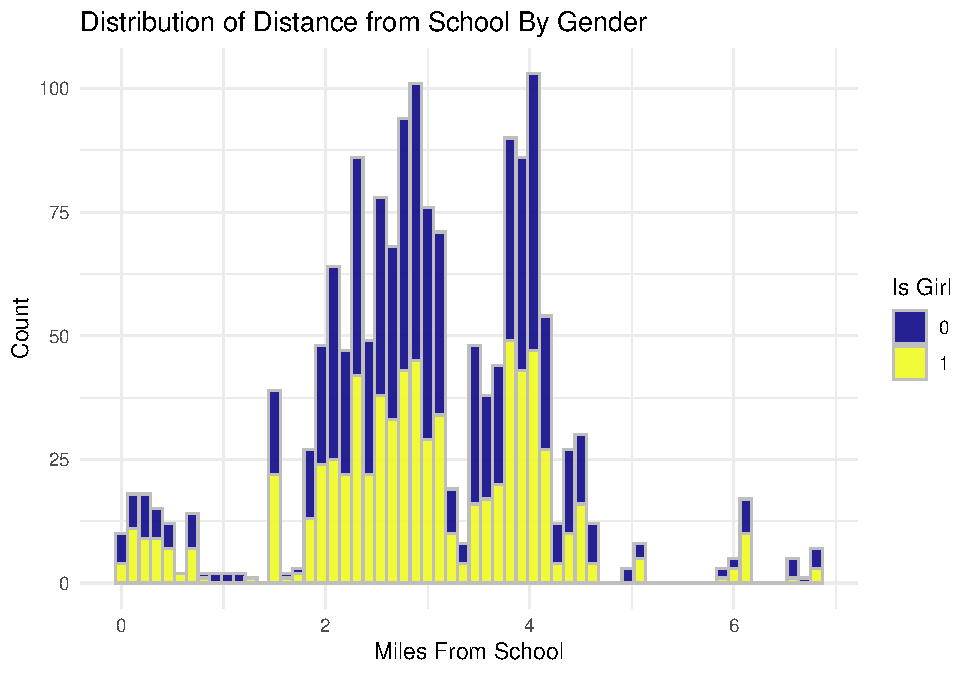
\includegraphics{HW1_files/figure-latex/histrogram-1.pdf}

\begin{Shaded}
\begin{Highlighting}[]
\FunctionTok{stargazer}\NormalTok{(reg3,reg4, }\AttributeTok{out =} \StringTok{"latex"}\NormalTok{, }\AttributeTok{dep.var.labels =} \StringTok{"Formal School"}
\NormalTok{          , }\AttributeTok{title =} \StringTok{"Column 1 and 2 With Outliers"}\NormalTok{, }\AttributeTok{header =}\NormalTok{ F)}
\end{Highlighting}
\end{Shaded}

\begin{table}[!htbp] \centering 
  \caption{Column 1 and 2 With Outliers} 
  \label{} 
\begin{tabular}{@{\extracolsep{5pt}}lcc} 
\\[-1.8ex]\hline 
\hline \\[-1.8ex] 
 & \multicolumn{2}{c}{\textit{Dependent variable:}} \\ 
\cline{2-3} 
\\[-1.8ex] & \multicolumn{2}{c}{Formal School} \\ 
\\[-1.8ex] & (1) & (2)\\ 
\hline \\[-1.8ex] 
 treatment & 0.510$^{***}$ & 0.386$^{***}$ \\ 
  & (0.087) & (0.099) \\ 
  & & \\ 
 chagcharan & 0.176$^{**}$ & 0.071 \\ 
  & (0.080) & (0.093) \\ 
  & & \\ 
 Constant & 0.082$^{*}$ & 0.321$^{***}$ \\ 
  & (0.049) & (0.057) \\ 
  & & \\ 
\hline \\[-1.8ex] 
Observations & 730 & 830 \\ 
R$^{2}$ & 0.325 & 0.171 \\ 
Adjusted R$^{2}$ & 0.323 & 0.169 \\ 
Residual Std. Error & 0.410 (df = 727) & 0.453 (df = 827) \\ 
\hline 
\hline \\[-1.8ex] 
\textit{Note:}  & \multicolumn{2}{r}{$^{*}$p$<$0.1; $^{**}$p$<$0.05; $^{***}$p$<$0.01} \\ 
\end{tabular} 
\end{table}

\newpage

\hypertarget{written-questions}{%
\section{\texorpdfstring{\textbf{Written
Questions:}}{Written Questions:}}\label{written-questions}}

\hypertarget{outlier-question-1}{%
\subsection{Outlier question 1:}\label{outlier-question-1}}

An outlier observation is someone who had more than 50 sheep or goats
owned by the household in 2007 and observed in the fall of 2007 or had
more than 10 jeribs of land owned by the household and was observed in
the fall of 2007 or had more than 20 people in the headcount in fall of
2007 or a person that has number of people in a household greater than
20 and are observed in summer of 2008. They are also an outlier if the
number of jeribs of land counted is more than 10 and are observed in
summer of 2008. Lastly if the number of sheep and goats is above 50 and
they are observed in summer of 2008.

\hypertarget{table-4-column-1-question-5}{%
\subsection{Table 4 Column 1 Question
5:}\label{table-4-column-1-question-5}}

Both of our coefficient estimates were very similar as the treatment for
girls and boys were exactly the same to the thousandth degree. The
standard error for women was exactly the same while the standard error
for men is unknown from table four.

\hypertarget{table-4-column-1-question-6}{%
\subsection{Table 4 Column 1 Question
6:}\label{table-4-column-1-question-6}}

The coefficients on all estimates are minimuly different with the
largest change being an increase in the treatment coefficient between
boys of .15. For women the coefficient decreased by .11 when including
outliers. The standard errors are also negligibly different.

\hypertarget{table-4-column-2-question-6}{%
\subsection{Table 4 Column 2 Question
6:}\label{table-4-column-2-question-6}}

Like in table 4, both treatments are statically significant. For girls,
the only statistically significant control is the child's age in the
fall of 2007 (5\%). For The males there were more statistically
significant controls. The age of the child, (1\% level) if the child's
family speaks Tajik, (5\% level) if the head of household is a farmer or
not, (10\% level) and lastly the nearest schools distance, (5\% level) .
For both genders the child's age was significant and positive which
means that as the child grows older, they are more likely to get a
better test score.

\hypertarget{further-analysis}{%
\subsection{Further Analysis:}\label{further-analysis}}

To start looking at the relationship at the between school we regressed
formal enrolled on the distance to the nearest school, whether the child
was a girl, an interaction between the two and a variables for distance
squared to control for any quadratic patterns. Surprisingly the only
statistically significant variable in that regression was whether or not
the child was a girl. This means that being farther away does not affect
formal enrollment and distance does not affect girls more than boys. The
regression output does implicate that women do attend school less than
their boy counterparts. Now when re-looking at formal enrollment based
on four distance types, short medium short, medium long, and long, we
can see that for girl, the amount of distance does not change the fact
that treatment is significantly increasing enrollment or test scores.
More specifically as distance increases, the effect of the treatment on
tests for girls decreases while it increases for men. Meaning that the
treatment is most effective for girls who live close and boys who live
farther away. Interestingly the treatment for both boys and girls are
mostly similar except when the schools were a medium long distance away
meaning that distance does not play a significant role in how the
treatment will affect the sexes. Overall it seems as though distance is
a more important variable when looking at the test scores for boys and
girls and not as much for their attendance rates.

\end{document}
